\documentclass[11pt,xcolor=table,aspectratio=169]{beamer}
\usepackage{babel}
\usetheme{metropolis}
\usepackage{appendixnumberbeamer}
\usepackage{booktabs}

\title[Biomedical sensors 20/21]{Embedded measurement systems development}
\subtitle{Development rundown}
\author{M. Pezzoli}
\date{A.Y. 2020-2021}
%\beamertemplatenavigationsymbolsempty
%\setbeamercovered{transparent} 
\usepackage{datetime2}
\usepackage{textpos}
\usepackage{pifont}
\usepackage{listings}
\newcommand{\cmark}{\ding{51}}%
\newcommand{\xmark}{\ding{55}}%


%Definizione colori
\definecolor{uniPVPink}{RGB}{157, 44, 73}
\definecolor{uniPVDarkBlue}{RGB}{14,12,24}
\definecolor{uniBGBlue}{RGB}{28,53,93}
\definecolor{paletteDarkGreen}{HTML}{4fa57a}
\definecolor{paletteLightGreen}{HTML}{9ee5b7}
\definecolor{uniBGLightBlue}{RGB}{148,177,223}
\definecolor{metropolisBackground}{RGB}{250,250,250}
\definecolor{orangeBeamer}{HTML}{FFD24A}

%Tikz
\usepackage{tikz}
\usetikzlibrary{automata,arrows.meta,shapes,calc,positioning,patterns,fit,3d,decorations.markings,matrix,spy,fadings,arrows}
\usepackage[americancurrents,arrowmos]{circuitikz}


\makeatletter
\tikzset{horizontal custom shading/.code={%
		\pgfmathsetmacro\tikz@vcs@middle{#1}
		\pgfmathsetmacro\tikz@vcs@bottom{\tikz@vcs@middle/2}
		\pgfmathsetmacro\tikz@vcs@top{(100-\tikz@vcs@middle)/2+\tikz@vcs@middle}
		\pgfdeclarehorizontalshading[tikz@axis@top,tikz@axis@middle,tikz@axis@bottom]{newaxis}{100bp}{%
			color(0bp)=(tikz@axis@bottom);
			color(\tikz@vcs@bottom bp)=(tikz@axis@bottom);
			color(\tikz@vcs@middle bp)=(tikz@axis@middle);
			color(\tikz@vcs@top bp)=(tikz@axis@top);
			color(100bp)=(tikz@axis@top)}
		\pgfkeysalso{/tikz/shading=newaxis}
	}
}
\makeatother  

\begin{tikzfadingfrompicture}[name=fade right]
	\shade[left color=transparent!5,middle color=transparent!5,
	right color=transparent!100] (0,0) rectangle (2,2);
\end{tikzfadingfrompicture}
%
\titlegraphic{
	\vspace{6cm}%
	\hspace{0.5cm}%
	
\includegraphics[height=1.4cm]{media/UniBG_logoComplete}
	\hspace{0.2cm}%
}

%\setbeamertemplate{frametitle}{%
%	\begin{beamercolorbox}{section in head/foot}
%		\vskip2pt\insertnavigation{\paperwidth}\vskip2pt
%	\end{beamercolorbox}%
%}
\tikzfading[name=fade right,left color=transparent!0,right color=transparent!100]
\setbeamertemplate{frametitle}{%
	\begin{tikzpicture}[remember picture,overlay]	
		%\fill[uniPVPink,path fading=fade right] (current page.north west) rectangle (\pagewidth, -.5cm);
		\fill[uniBGBlue!95](current page.north west) rectangle (\paperwidth ,-.5cm);
		\node[anchor=center] (logo) at (.89\paperwidth,0){
\includegraphics[height=.91cm,width=.91cm]{media/UniBG_logo}};
		\node[align=left,anchor=west](title) at (-.05\paperwidth,0){\insertframetitle};	
	\end{tikzpicture}%
\vskip15pt
}


% Numeri di pagina
\defbeamertemplate*{footline}{shadow theme}
{
	\leavevmode
	\hbox{\begin{beamercolorbox}[wd=.25\paperwidth,ht=2.1ex,dp=1.125ex,leftskip=.3cm plus1fil,rightskip=.3cm]{author in head/foot}%
			\usebeamerfont{author in head/foot}\insertframenumber\,/\,\inserttotalframenumber\hfill\insertshortauthor
		\end{beamercolorbox}
		\begin{beamercolorbox}[wd=.5\paperwidth,ht=2.1ex,dp=1.125ex,leftskip=.3cm,rightskip=.3cm plus1fil]{title in head/foot}
			\usebeamerfont{title in head/foot}\insertshorttitle
	\end{beamercolorbox}}
	\vskip0pt
}

\setbeamercolor*{palette primary}{use=structure,fg=white,bg=uniBGBlue}
\setbeamercolor{frametitle}{fg=white,bg=uniBGBlue}
\setbeamercolor{title separator}{bg=white,fg=uniBGBlue}
\setbeamercolor{structure}{fg=uniBGBlue,bg=white}
\setbeamercolor{alerted text}{fg=uniBGBlue}
\setbeamercolor{block title}{fg=uniBGBlue,bg=uniBGBlue!15}
% Figure
\usepackage{graphicx}
\usepackage{epstopdf}
\DeclareGraphicsExtensions{.eps,.png,.jpg,.pdf}
\usepackage{float}

\usepackage{makecell}



% Pacchetti matematica
\usepackage{amsmath}
\usepackage{amsthm}
\usepackage{amssymb}
\usepackage{mathtools}



\tikzset{
	set arrow inside/.code={\pgfqkeys{/tikz/arrow inside}{#1}},
	set arrow inside={end/.initial=>, opt/.initial=},
	/pgf/decoration/Mark/.style={
		mark/.expanded=at position #1 with
		{
			\noexpand\arrow[\pgfkeysvalueof{/tikz/arrow inside/opt}]{\pgfkeysvalueof{/tikz/arrow inside/end}}
		}
	},
	arrow inside/.style 2 args={
		set arrow inside={#1},
		postaction={
			decorate,decoration={
				markings,Mark/.list={#2}
			}
		}
	},
}

\definecolor{plotColor1}{RGB}{55,126,184}
\definecolor{plotColor2}{RGB}{228,26,28}
\definecolor{plotColor3}{RGB}{255,127,0}
\definecolor{plotColor4}{RGB}{152,78,163}
\definecolor{plotColor5}{RGB}{77,174,74}
\definecolor{plotColor6}{RGB}{255,255,51}
\definecolor{plotColor7}{RGB}{166,86,40}
\definecolor{plotColor8}{RGB}{247,129,191}
\definecolor{plotColor9}{RGB}{153,153,153}



\definecolor{grad1}{HTML}{FF0000}
\definecolor{grad2}{HTML}{FF5700}
\definecolor{grad3}{HTML}{FEAD00}
\definecolor{grad4}{HTML}{F9FE00}
\definecolor{grad5}{HTML}{A2FE00}
\definecolor{grad6}{HTML}{00FB0D}
\definecolor{grad7}{HTML}{00FD61}
\definecolor{grad8}{HTML}{00FCB6}
\definecolor{grad9}{HTML}{00ECFC}
\definecolor{grad10}{HTML}{0096FC}
\definecolor{grad11}{HTML}{0041FB}
\definecolor{grad12}{HTML}{1500FB}

%\definecolor{plotColor1}{RGB}{166,206,227}
%\definecolor{plotColor2}{RGB}{31,120,180}
%\definecolor{plotColor3}{RGB}{178,223,138}
%\definecolor{plotColor4}{RGB}{51,160,44}
%\definecolor{plotColor5}{RGB}{251,154,153}
%\definecolor{plotColor6}{RGB}{227,26,28}
%\definecolor{plotColor7}{RGB}{253,191,111}
%\definecolor{plotColor8}{RGB}{255,127,0}
%\definecolor{plotColor9}{RGB}{202,178,214}
%\definecolor{plotColor10}{RGB}{106,61,154}
%\definecolor{plotColor11}{RGB}{255,255,153}
%\definecolor{plotColor12}{RGB}{177,89,40}
%\definecolor{plotColor13}{RGB}{}
%\definecolor{plotColor14}{RGB}{}
%\definecolor{plotColor15}{RGB}{}
%\definecolor{plotColor16}{RGB}{}
%\definecolor{plotColor17}{RGB}{}
%\definecolor{plotColor18}{RGB}{}

%Pgrplots
\usepackage{pgfplots}
\usepackage[binary-units=true]{siunitx}
%\pgfplotsset{compat=newest}
\usepgfplotslibrary{units,groupplots,fillbetween}
\pgfplotscreateplotcyclelist{myColorList}{
	{plotColor1},
	{plotColor2},
	{plotColor3},
	{plotColor4},
	{plotColor5},
	{plotColor6},
	{plotColor7},
	{plotColor8},
	{plotColor9},
}

\pgfplotscreateplotcyclelist{slines}{
	{thin,solid},
	{thin,densely dashed},
	{thick,densely dotted},
	{thick,solid},
	{very thick,densely dashed},
	{very thick,densely dashdotdotted},
}
\pgfplotsset{
	every mark/.append style={fill={}},
	% Cycle list styles ----------------------------------------
	style colors/.style={cycle list name=myColorList},
	style lines/.style={cycle multiindex* list={myColorList\nextlist slines}},
	style marks/.style={cycle multiindex* list={myColorList\nextlist mark list*}},
	% Graph styles ---------------------------------------------
	graph/.style={grid=both,style #1},
	graph/.default={lines},
}


\usepackage{pgfplotstable}
%per ridimensionare le picture
\usepackage{adjustbox}
\usepackage{eurosym}

\DeclareSIUnit{\pers}{pers}
\DeclareSIUnit{\EUR}{\text{\euro}}
\sisetup{
	per-mode = fraction,
	inter-unit-product = \ensuremath{{}\cdot{}},
}
\usepackage{filecontents}





%BEGIN_FOLD Custom tikz shapes
%BEGIN_FOLD Custom PMOS
\pgfdeclareshape{customPMOS}{
	\anchor{center}{\pgfpointorigin}
	\anchor{text}{\pgfpoint{-.5\wd\pgfnodeparttextbox}{-.5\ht\pgfnodeparttextbox}}
	\savedanchor\mosS{\pgfpoint{.293cm}{.193cm}} % Source
	\anchor{S}{\mosS}
	\savedanchor\mosD{\pgfpoint{.293cm}{-.193cm}} % Drain
	\anchor{D}{\mosD}
	\savedanchor\mosG{\pgfpoint{-.45cm}{0}} % Gate
	\anchor{G}{\mosG}
	\savedanchor\mosB{\pgfpoint{0}{0}} % Bulk
	\anchor{B}{\mosB}
	\foregroundpath
	{ 
		\pgfsetlinewidth{0.014cm}\pgfpathmoveto{\pgfpoint{-.45cm}{0}}\pgfpathlineto{\pgfpoint{-.13cm}{0}}\pgfusepath{stroke}
		\pgfsetlinewidth{0.014cm}\pgfpathcircle{\pgfpoint{-.13cm}{0}}{.04cm}\pgfsetfillcolor{white}\pgfusepath{fill,stroke}
		\pgfsetlinewidth{0.05cm}\pgfpathmoveto{\pgfpoint{-.065cm}{.22cm}}\pgfpathlineto{\pgfpoint{-.065cm}{-.22cm}}\pgfusepath{stroke}
		\pgfsetlinewidth{0.014cm}\pgfpathmoveto{\pgfpoint{.3cm}{.2cm}}\pgfsetarrowsend{Triangle[length=1.5pt,angle'=30]}\pgfpathlineto{\pgfpoint{0}{.2cm}}\pgfusepath{stroke}
		\pgfsetarrowsend{}
		\pgfpathmoveto{\pgfpoint{0}{.22cm}}\pgfpathlineto{\pgfpoint{0}{-.22cm}}\pgfpathmoveto{\pgfpoint{0}{-.2cm}}\pgfpathlineto{\pgfpoint{.3cm}{-.2cm}}\pgfusepath{stroke}
	}
}
%END_FOLD
%BEGIN_FOLD Custom NMOS
\pgfdeclareshape{customNMOS}{
	\anchor{center}{\pgfpointorigin}
	\anchor{text}{\pgfpoint{-.5\wd\pgfnodeparttextbox}{-.5\ht\pgfnodeparttextbox}}
	\savedanchor\mosS{\pgfpoint{.293cm}{.193cm}} % Drain
	\anchor{S}{\mosS}
	\savedanchor\mosD{\pgfpoint{.293cm}{-.193cm}} % Source
	\anchor{D}{\mosD}
	\savedanchor\mosG{\pgfpoint{-.45cm}{0}} % Gate
	\anchor{G}{\mosG}
	\savedanchor\mosB{\pgfpoint{0}{0}} % Bulk
	\anchor{B}{\mosB}
	\foregroundpath
	{ 
		\pgfsetlinewidth{0.014cm}\pgfpathmoveto{\pgfpoint{-.45cm}{0}}\pgfpathlineto{\pgfpoint{-.065cm}{0}}\pgfusepath{stroke}
		\pgfsetlinewidth{0.05cm}\pgfpathmoveto{\pgfpoint{-.065cm}{.22cm}}\pgfpathlineto{\pgfpoint{-.065cm}{-.22cm}}\pgfusepath{stroke}
		\pgfsetlinewidth{0.014cm}\pgfpathmoveto{\pgfpoint{0}{-.2cm}}\pgfsetarrowsend{Triangle[length=1.5pt,angle'=30]}\pgfpathlineto{\pgfpoint{.3}{-.2cm}}\pgfsetarrowsend{}\pgfusepath{stroke}
		\pgfpathmoveto{\pgfpoint{0}{-.22cm}}\pgfpathlineto{\pgfpoint{0}{.22cm}}\pgfpathmoveto{\pgfpoint{0}{.2cm}}\pgfpathlineto{\pgfpoint{.3cm}{.2cm}}\pgfusepath{stroke}
	}
}
%END_FOLD
%BEGIN_FOLD Custom controlled switch (negated logic)
\pgfdeclareshape{customVCSwitchN}{
	\anchor{center}{\pgfpointorigin}
	\anchor{text}{\pgfpoint{-.5\wd\pgfnodeparttextbox}{-.5\ht\pgfnodeparttextbox}}
	\savedanchor\sIN{\pgfpoint{-.35cm}{0}} % IN1
	\anchor{INA}{\sIN}
	\savedanchor\sOUT{\pgfpoint{.35cm}{0}} % IN2
	\anchor{INB}{\sOUT}
	\savedanchor\sCTRL{\pgfpoint{0}{.293cm}} % Control
	\anchor{CTRL}{\sCTRL}
	\foregroundpath
	{ 
		\pgfsetlinewidth{0.014cm}
		\pgfpathmoveto{\pgfpoint{.35cm}{0}}\pgfpathlineto{\pgfpoint{.12cm}{0}}\pgfpathlineto{\pgfpointpolar{150}{.14cm}}
		\pgfpathmoveto{\pgfpoint{-.12cm}{0}}\pgfpathlineto{\pgfpoint{-.35cm}{0}}
		\pgfpathrectanglecorners{\pgfpoint{-.2cm}{-.075cm}}{\pgfpoint{.2cm}{.15cm}}
		\pgfpathmoveto{\pgfpoint{0}{.23cm}}\pgfpathlineto{\pgfpoint{0}{.3cm}}
		\pgfusepath{stroke}
		
		\pgfsetlinewidth{0.015cm}
		\pgfpathcircle{\pgfpoint{0}{.19cm}}{.04cm}
		\pgfsetfillcolor{white}
		\pgfusepath{fill,stroke}
	}
}
%END_FOLD
%BEGIN_FOLD Custom external signal switch
\pgfdeclareshape{customExtVCSwitch}{
	\anchor{center}{\pgfpointorigin}
	\anchor{text}{\pgfpointdiff{\pgfpoint{.5\wd\pgfnodeparttextbox}{.5\ht\pgfnodeparttextbox}}{\pgfpoint{0}{.6cm}}}	
	\savedanchor\sIN{\pgfpoint{-.35cm}{0}} % IN1
	\anchor{INA}{\sIN}
	\savedanchor\sOUT{\pgfpoint{.35cm}{0}} % IN2
	\anchor{INB}{\sOUT}
	\savedanchor\sNAME{\pgfpointadd{\pgfpoint{-.5\wd\pgfnodeparttextbox}{-.5\ht\pgfnodeparttextbox}}{\pgfpoint{0}{.5cm}}} % Signal name
	\anchor{NAME}{\sNAME}
	
	\foregroundpath
	{ 
		\pgfsetlinewidth{0.015cm}
		\pgfpathmoveto{\pgfpoint{.35cm}{0}}\pgfpathlineto{\pgfpoint{.12cm}{0}}\pgfpathlineto{\pgfpointpolar{150}{.14cm}}
		\pgfpathmoveto{\pgfpoint{-.12cm}{0}}\pgfpathlineto{\pgfpoint{-.35cm}{0}}
		\pgfpathrectanglecorners{\pgfpoint{-.2cm}{-.075cm}}{\pgfpoint{.2cm}{.15cm}}
		\pgfpathmoveto{\pgfpoint{0}{.15cm}}\pgfpathlineto{\pgfpoint{0}{.3cm}}
		\pgfusepath{stroke}
		
		\pgfpathmoveto{\pgfpoint{0cm}{.28cm}}\pgfpathlineto{\pgfpoint{.05cm}{.35cm}}\pgfpathlineto{\pgfpoint{.05cm}{.45cm}}\pgfpathlineto{\pgfpoint{-.05cm}{.45cm}}\pgfpathlineto{\pgfpoint{-.05cm}{.35cm}}
		\pgfsetfillcolor{black}
		\pgfusepath{fill}
	}
}
%END_FOLD
%BEGIN_FOLD Custom external signal switch (negated logic)
\pgfdeclareshape{customExtVCSwitchN}{
	\anchor{center}{\pgfpointorigin}
	\anchor{text}{\pgfpointdiff{\pgfpoint{.5\wd\pgfnodeparttextbox}{.5\ht\pgfnodeparttextbox}}{\pgfpoint{0}{.6cm}}}
	\savedanchor\sIN{\pgfpoint{-.35cm}{0}} % IN1
	\anchor{INA}{\sIN}
	\savedanchor\sOUT{\pgfpoint{.35cm}{0}} % IN2
	\anchor{INB}{\sOUT}
	\savedanchor\sNAME{\pgfpointadd{\pgfpoint{-.5\wd\pgfnodeparttextbox}{-.5\ht\pgfnodeparttextbox}}{\pgfpoint{0}{.5cm}}} % Signal name
	\anchor{NAME}{\sNAME}
	
	\foregroundpath
	{ 
		\pgfsetlinewidth{0.015cm}
		\pgfpathmoveto{\pgfpoint{.35cm}{0}}\pgfpathlineto{\pgfpoint{.12cm}{0}}\pgfpathlineto{\pgfpointpolar{150}{.14cm}}
		\pgfpathmoveto{\pgfpoint{-.12cm}{0}}\pgfpathlineto{\pgfpoint{-.35cm}{0}}
		\pgfpathrectanglecorners{\pgfpoint{-.2cm}{-.075cm}}{\pgfpoint{.2cm}{.15cm}}
		\pgfpathmoveto{\pgfpoint{0}{.23cm}}\pgfpathlineto{\pgfpoint{0}{.3cm}}
		\pgfusepath{stroke}
		
		\pgfpathmoveto{\pgfpoint{0cm}{.28cm}}\pgfpathlineto{\pgfpoint{.05cm}{.35cm}}\pgfpathlineto{\pgfpoint{.05cm}{.45cm}}\pgfpathlineto{\pgfpoint{-.05cm}{.45cm}}\pgfpathlineto{\pgfpoint{-.05cm}{.35cm}}
		\pgfsetfillcolor{black}
		\pgfusepath{fill}
		
		\pgfsetlinewidth{0.015cm}
		\pgfpathcircle{\pgfpoint{0}{.19cm}}{.04cm}
		\pgfsetfillcolor{white}
		\pgfusepath{fill,stroke}
	}	
}
%END_FOLD
%BEGIN_FOLD Custom input
\pgfdeclareshape{customINSignal}{
	\anchor{center}{\pgfpointorigin}
	\anchor{text}{\pgfpointadd{\pgfpoint{-\wd\pgfnodeparttextbox}{-.5\ht\pgfnodeparttextbox}}{\pgfpoint{-.23cm}{0cm}}}
	\savedanchor\wire{\pgfpoint{-.1cm}{0}} % Wire
	\anchor{W}{\wire}
	\foregroundpath
	{ 
		\pgfpathmoveto{\pgfpoint{0cm}{0cm}}\pgfpathlineto{\pgfpoint{-.05cm}{.05cm}}\pgfpathlineto{\pgfpoint{-.20cm}{.05cm}}\pgfpathlineto{\pgfpoint{-.20cm}{-.05cm}}\pgfpathlineto{\pgfpoint{-.05cm}{-.05cm}}
		\pgfsetfillcolor{black}
		\pgfusepath{fill}
		
	}
}
%END_FOLD
%BEGIN_FOLD Custom output
\pgfdeclareshape{customOUTSignal}{
	\anchor{center}{\pgfpointorigin}
	\anchor{text}{\pgfpointadd{\pgfpoint{-.5\wd\pgfnodeparttextbox}{-.5\ht\pgfnodeparttextbox}}{\pgfpoint{-.23cm}{0cm}}}
	\savedanchor\wire{\pgfpoint{-.1cm}{0}} % Wire
	\anchor{W}{\wire}
	\foregroundpath
	{ 
		\pgfpathmoveto{\pgfpoint{0cm}{0cm}}\pgfpathlineto{\pgfpoint{0cm}{.05cm}}\pgfpathlineto{\pgfpoint{-.15cm}{.05cm}}\pgfpathlineto{\pgfpoint{-.20cm}{0cm}}\pgfpathlineto{\pgfpoint{-.15cm}{-.05cm}}\pgfpathlineto{\pgfpoint{0cm}{-.05cm}}
		\pgfsetfillcolor{black}
		\pgfusepath{fill}
		
	}
}
%END_FOLD

%BEGIN_FOLD Custom arrows
\tikzstyle{vecArrow} = [thick, decoration={markings,mark=at position1 with {\arrow[semithick]{open triangle 60}}},double distance=1.4pt, shorten >= 5.5pt,preaction = {decorate},postaction = {draw,line width=1.4pt, white,shorten >= 4.5pt}]
\tikzstyle{innerWhite} = [semithick, white,line width=1.4pt, shorten >= 4.5pt]
%END_FOLD

%END_FOLD

\definecolor{mDarkTeal}{HTML}{23373b}
\usepackage{appendixnumberbeamer}

\begin{document}
	
	\maketitle
	\begin{frame}
		\frametitle{Introduction}
		The goal of this last part of the Biomedical sensors course is to give some insights in the development of embedded measurement systems. The topics covered will be:
		\begin{itemize}
			\item project phase: specs definition, sensors and components selection;
			\item PCB design and manufacture;
			\item firmware development
			\item one or more case studies in the biomedical field.
		\end{itemize}
	\end{frame}

	\begin{frame}
		\frametitle{Challenges}
		Typical embedded system challenges:
		\begin{itemize}
			\item \textbf{Small size, low weight}\begin{itemize}
				\item Handheld electronics
				\item Transport cost
			\end{itemize}
			\item \textbf{Low power} \begin{itemize}
				\item Battery powered for 8+ hours
				\item Small size means small thermal dissipation capabilities
			\end{itemize}
			\item \textbf{Safety critical operation}\begin{itemize}
				\item Embedded systems work in danger-prone environments (Industrial, Biomedical, ...)
			\end{itemize}
			\item \textbf{Cost sensitivity}
		\end{itemize}
	\end{frame}

	\begin{frame}
		\frametitle{Project phase - Outline}
		\textbf{Goal:} make all the components and architectural choices to lay the groundwork for the design phase.
		\begin{columns}
			\begin{column}{.5\textwidth}
				\begin{itemize}
					\item Specs draft.
					\item Sensors alternatives.
					\item Microcontroller alternatives.
				\end{itemize}
			\end{column}
			\begin{column}{.5\textwidth}
				\begin{itemize}
					\item Memory requirements.
					\item Communication requirements.
					\item System-related components.
				\end{itemize}
			\end{column}
		\end{columns}
	\end{frame}

	\begin{frame}
		\frametitle{Project phase - Specifications draft}
		The \textbf{specification document} is the \textbf{basic foundation} of a good project. Well defined specs make components choices trivial work; the engineer's job is to \textbf{make abstract requests into requirements} that fit into the specs document.
		\vspace{.05cm}
		\begin{center}
			\begin{tabular}{ccc}
				\makecell{\textbf{Gait analysis}\\\textbf{system}}  & $\longrightarrow$ & \makecell{\textbf{Accelerometer}: at least \SIrange{5}{8}{g} full scale\\ \textbf{Weight}: to minimize}
			\end{tabular}
		\end{center}
		Inside the specifications document:
		\begin{itemize}
			\item Measurements specifications (e.g. accuracy, frequency, full scale...).
			\item Data specifications (e.g. memory, communication, computation on data...).
			\item System specifications (e.g. power supply, life time, future expansions...).
			\item Mechanical specifications (e.g. dimensions, weight, mounting holes...).		
		\end{itemize}
	\end{frame}

	\begin{frame}
		\frametitle{Project phase - Common parameters}
		Keep in mind characteristics that MUST be considered for every component, even if not mentioned in later slides:
		\begin{description}
			\item[Power consumption] embedded systems thrive on energy efficiency; power consumption should always be considered when choosing any component or making design choices.
			\item[Size] an embedded system has the goal of performing complex operation in a small form factor;
			\item[Cost] if the system needs to go to the consumer market, cost will play a big role in the choice of components;
			\item[Peripheral used] always keep in mind what microcontroller peripherals the component will require; avoid choices that will overhaul your microcontroller choice.
		\end{description}
	\end{frame}

	\begin{frame}
		\frametitle{Project phase - Microcontroller alternatives}
		\only<1>{
			\textbf{M}icro\textbf{C}ontroller \textbf{U}nit: a programmable device that can perform complex operations. Made up by (simplifying) one or more cores (CPU), memory and I/O peripherals, besides other support peripherals.\\
			Generally speaking, microcontroller functions are that of \textbf{input}, \textbf{computation}, \textbf{output} and \textbf{communication}.\\\vspace{.3cm}
			\begin{center}
				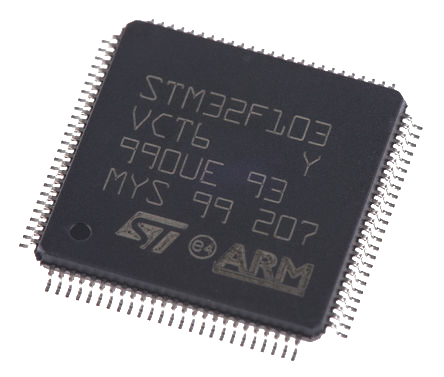
\includegraphics[width=.3\paperwidth]{media/micro.png}
			\end{center}
		}
		\only<2>{
			What to look for when choosing a microcontroller:
			\begin{itemize}
				\item Addressing size/bits (8, 16, 32 bits)
				\item Architecture (ARM, x86, ...)
				\item[\textcolor{orangeBeamer}{\textbullet}] \textbf{F}loating \textbf{P}oint \textbf{U}nit
				\item[\textcolor{orangeBeamer}{\textbullet}] Memory size
				\item[\textcolor{orangeBeamer}{\textbullet}] Appropriate peripherals
				\item[\textcolor{orangeBeamer}{\textbullet}] Mechanical dimensions
				\item[\textcolor{orangeBeamer}{\textbullet}] Power consumption
			\end{itemize}
		}
	\end{frame}

	\begin{frame}
		\frametitle{Microcontroller intermission - Non-volatile memory}
		\begin{columns}
			\begin{column}{.6\textwidth}
				Memory used to save data that needs to persist even without power, usually in the \SIrange{0.2}{2}{\mega\byte} range, implemented as a flash memory (like USB sticks).\\
				It is used to save:
				\begin{itemize}
					\item microcontroller program logic
					\item user data needed between boots (configuration)
					\item option bytes
				\end{itemize}
			\end{column}
			\begin{column}{.3\textwidth}
				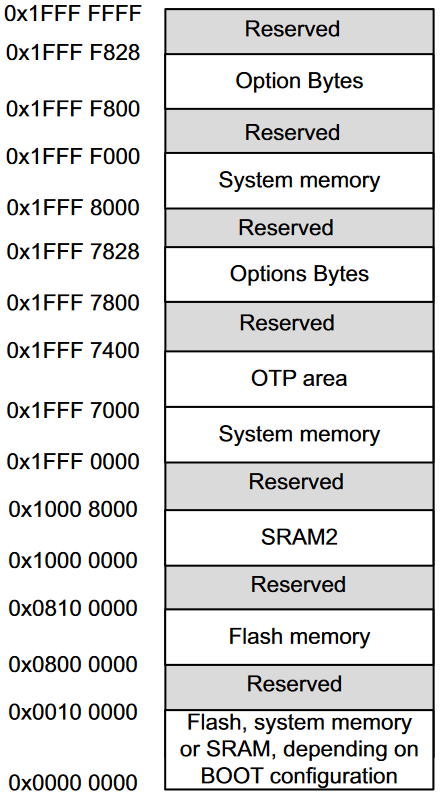
\includegraphics[width=.72\textwidth]{media/flash.PNG}
			\end{column}
		\end{columns}
	\end{frame}
	
	\begin{frame}
		\frametitle{Microcontroller intermission - Volatile memory}
		Memory used to save temporary data; said data do not persist without power. Usually in the \SI{50}{\kilo\byte} to \SI{1}{\mega\byte} range.
		Often implemented as RAM, it is used to contain program data during execution:
			\begin{itemize}
				\item stack
				\item heap
			\end{itemize}
		\vspace{.2cm}
		Configuration and interface between CPU and memory lead to an architectural differentiation:
		\begin{itemize}
			\item von Neumann
			\item Harvard
		\end{itemize}
	\end{frame}
	
	\begin{frame}
	\frametitle{Microcontroller intermission - Von Neumann architecture}
		Von Neumann architecture provides a single bus that feeds data AND code to the CPu. Code and data MUST share the same address space.
		\begin{columns}
			\begin{column}{.6\textwidth}
				\begin{itemize}
					\item[\cmark] Simpler hardware
					\item[\cmark] More efficient memory use
					\item[\xmark] Possible conflicts between data and code
					\item[\xmark] Bottleneck in the bus
				\end{itemize}
			\end{column}
			\begin{column}{.4\textwidth}
				\centering
				\begin{adjustbox}{max width=\textwidth}
					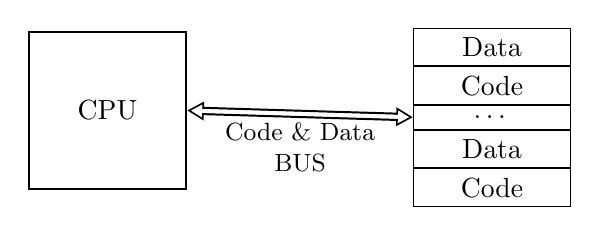
\begin{tikzpicture}
						\node (CPU) at (0,0) [draw,thick,minimum width=2cm,minimum height=2cm,anchor=center] {CPU};
						\node (mem) at (4,-1.1){};
						\node (code) at (mem.south west)[draw, minimum width=2cm, minimum height=.3cm,anchor=south west]{Code};
						\node (data) at (code.north west)[draw, minimum width=2cm, minimum height=.3cm,anchor=south west]{Data};
						\node (dots) at (data.north west)[draw, minimum width=2cm, minimum height=.3cm,anchor=south west]{$\dots$};
						\node (code1) at (dots.north west)[draw, minimum width=2cm, minimum height=.3cm,anchor=south west]{Code};
						\node (data1) at (code1.north west)[draw, minimum width=2cm, minimum height=.3cm,anchor=south west]{Data};
						
						\draw[vecArrow] ($(CPU.east)!.5!(dots.west)$) --(CPU.east);
						\draw[vecArrow] ($(CPU.east)!.5!(dots.west)$) --(dots.west); 
						\node[below, align=center,font=\small] (t) at ($(CPU.east)!.5!(dots.west)$){Code \& Data\\BUS};
					\end{tikzpicture}
				\end{adjustbox}
			\end{column}
		\end{columns}
	\end{frame}
	
	\begin{frame}
		\frametitle{Microcontroller intermission - Harvard architecture}
		Harvard architecture provides dedicated buses for data and code. Data and code MAY share the same address space.
		\begin{columns}
			\begin{column}{.6\textwidth}
				\begin{itemize}
				\item[\cmark] Better performances
				\item[\cmark] Can have different sizes for instructions and data
				\item[\xmark] More complex hardware
				\end{itemize}
			\end{column}
			\begin{column}{.4\textwidth}
				\centering
				\begin{adjustbox}{max width=\textwidth}
					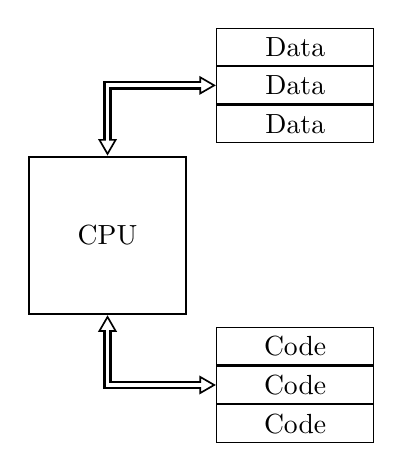
\begin{tikzpicture}
						\node (CPU) at (0,0) [draw,thick,minimum width=2cm,minimum height=2cm,anchor=center] {CPU};
						\node (mem) at ($(CPU.south)+(1.5,-1.5)$){};
						\node (mem1) at ($(CPU.north)+(1.5,1.5)$){};
						\node (code) at (mem.south west)[draw, minimum width=2cm, minimum height=.3cm,anchor=south west]{Code};
						\node (code1) at (code.north west)[draw, minimum width=2cm, minimum height=.3cm,anchor=south west]{Code};
						\node (code2) at (code1.north west)[draw, minimum width=2cm, minimum height=.3cm,anchor=south west]{Code};
						
						\node (data) at (mem1.north west)[draw, minimum width=2cm, minimum height=.3cm,anchor=north west]{Data};
						\node (data1) at (data.south west)[draw, minimum width=2cm, minimum height=.3cm,anchor=north west]{Data};
						\node (data2) at (data1.south west)[draw, minimum width=2cm, minimum height=.3cm,anchor=north west]{Data};
						
						\draw[vecArrow] ($(code1.west)+(-.5,0)$) -| (CPU.south);
						\draw[vecArrow] ($(CPU.south)+(0,-.5)$) |- (code1.west);
						\draw[vecArrow] ($(data1.west)+(-.5,0)$) -| (CPU.north);
						\draw[vecArrow] ($(CPU.north)+(0,.5)$) |- (data1.west);
					\end{tikzpicture}
				\end{adjustbox}
			\end{column}
		\end{columns}
	\end{frame}

	\begin{frame}
		\frametitle{Project phase - ST Cortex M line}
		\centering
		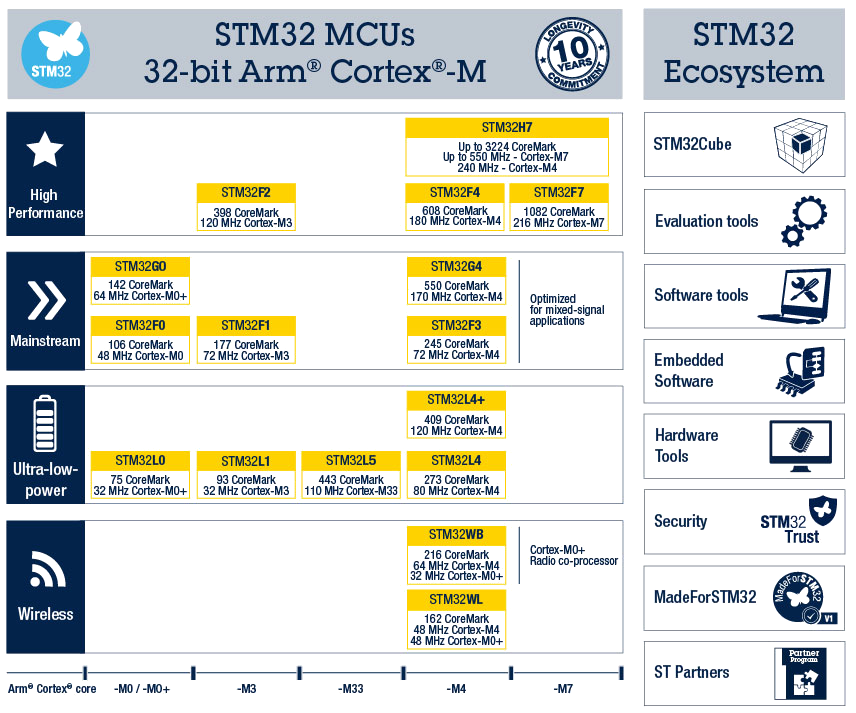
\includegraphics[width=.65\textwidth]{media/STCortex_small.png}
	\end{frame}

	\begin{frame}
		\frametitle{Peripheral intermission - ADC}
		\only<1>{
			\textbf{A}nalog to \textbf{D}igital \textbf{C}onverter: \textbf{digitalizes an analog signal} so that it can be trated digitally (in a firmware), or so that it can be transmitted.\\ An ADC is defined by its \textbf{bit count}, which determines the width of the converted digital word; the number of bits is strictly related to the error in the conversion from analog (continuous domain) to digital (discrete domain).\\
			\vspace{.3cm}
			\begin{center}
				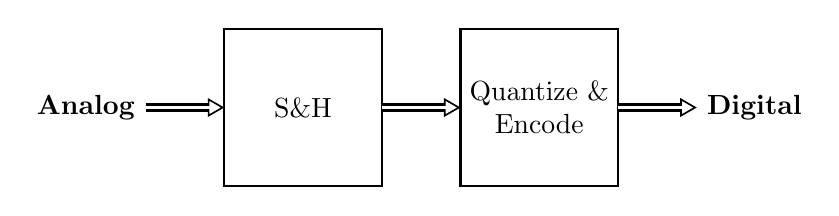
\begin{tikzpicture}
				\draw[thick] (0,0) rectangle (2,2) node[pos=.5]{S\&H};
				\draw[vecArrow] (2,1) -- (3,1);
				\draw[thick] (3,0) rectangle (5,2) node[pos=.5,align=center]{Quantize \&\\ Encode};
				\draw[vecArrow] (-1,1)node[anchor=east]  {\textbf{Analog}} -- ++(1,0);
				\draw[vecArrow] (5,1) -- ++(1,0)node[anchor=west]{\textbf{Digital}}; 
				\end{tikzpicture}
			\end{center}
		}
		\only<2>{
			\begin{columns}
				\begin{column}{.45\textwidth}
					The quantization phase compares the signal with discrete references in the domain (quanta), then encodes the result into a binary word. A \textbf{higher number of bits} leads to a \textbf{lower error of quantization}.
				\end{column}
				\begin{column}{.55\textwidth}
					\centering
					\begin{tikzpicture}
					\begin{axis}[xmin=0,xmax=8,ymax=8,ymin=0,xlabel={Digital domain},xtick={0,1,2,3,4,5,6,7},minor x tick num=1,xticklabels={000,001,010,011,100,101,110,111},height=.7\textheight,ylabel={Analog domain},label style={font=\small},every tick label/.append style={font=\tiny},yticklabels={},ytick={}]
					\addplot[const plot,uniPVPink] coordinates {(0,0) (.5,1) (1.5,2) (2.5,3) (3.5,4) (4.5,5) (5.5,6) (6.5,7)(8,7)};
					\addplot[uniBGBlue,domain=0:8]{x}; 
					\path[name path=axis] (axis cs:0,0) --(axis cs:8,0);
					\path[name path=top] (axis cs:0,8) -- (axis cs:8,8);
					\addplot[fill=uniBGBlue, fill opacity=0.06]fill between[of=top and axis,soft clip={domain=0:0.5}];
					\addplot[fill=uniBGBlue, fill opacity=0.12]fill between[of=axis and top,soft clip={domain=0.5:1.5}];
					\addplot[fill=uniBGBlue, fill opacity=0.06]fill between[of=top and axis,soft clip={domain=1.5:2.5}];
					\addplot[fill=uniBGBlue, fill opacity=0.12]fill between[of=top and axis,soft clip={domain=2.5:3.5}];
					\addplot[fill=uniBGBlue, fill opacity=0.06]fill between[of=top and axis,soft clip={domain=3.5:4.5}];
					\addplot[fill=uniBGBlue, fill opacity=0.12]fill between[of=top and axis,soft clip={domain=4.5:5.5}];
					\addplot[fill=uniBGBlue, fill opacity=0.06]fill between[of=top and axis,soft clip={domain=5.5:6.5}];
					\addplot[fill=uniBGBlue, fill opacity=0.12]fill between[of=top and axis,soft clip={domain=6.5:8}];
					
					\end{axis}	
					\end{tikzpicture}
				\end{column}
			\end{columns}
		}
	\end{frame}

	\begin{frame}
		\frametitle{Peripheral intermission - $I^2C$}
		\only<1>{
				\textbf{I}nter-\textbf{I}ntegrated \textbf{C}ircuits: syncronous serial bus for low speed (wired, short range) communication (up to some \si{\mega\hertz}). Usually in a master+multi-slave configuration, it has a 2-wire implementation (clock and data).\\\vspace{.5cm}
			\begin{columns}[T]
				\begin{column}{.7\textwidth}
					Typical transmission frequencies:
					\begin{itemize}
						\item Standard mode, \SI{100}{\kilo\hertz} clock
						\item Fast mode, \SI{400}{\kilo\hertz} clock
						\item Newer modes implement higher clock rates (\SI{1}{\mega\hertz}, \SI{5}{\mega\hertz})
					\end{itemize}
				\end{column}
				\begin{column}{.2\textwidth}
					\hspace{-3.3cm}
					\begin{adjustbox}{max width=1.8\textwidth}
						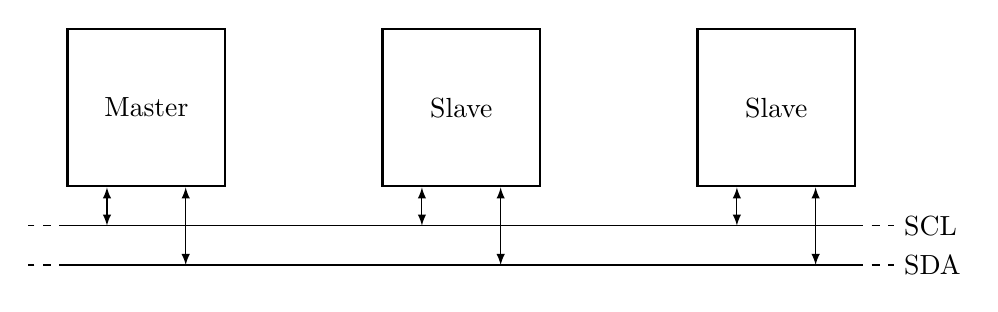
\begin{tikzpicture}
						\node (master) at (0,0) [draw,thick,minimum width=2cm,minimum height=2cm,anchor=center] {Master};
						\node (slave1) at (4,0) [draw,thick,minimum width=2cm,minimum height=2cm,anchor=center,align=center] {Slave};
						\node (slave2) at (8,0) [draw,thick,minimum width=2cm,minimum height=2cm,anchor=center] {Slave};
						\draw (-1,-1.5)coordinate (A) -- ++(10,0) (-1,-2)coordinate (B) -- ++(10,0);
						\draw [dashed] (-1,-1.5) -- ++(-.5,0) (9,-1.5) -- ++(.5,0) node[anchor=west]{SCL};
						\draw [dashed] (-1,-2) -- ++(-.5,0) (9,-2) -- ++(.5,0) node[anchor=west]{SDA};
						\draw[latex-latex] ($(master.south)+(-.5,0)$) coordinate (T1) -- (T1|-A); 
						\draw[latex-latex] ($(master.south)+(.5,0)$) coordinate (T2) -- (T2|-B);
						\draw[latex-latex] ($(slave1.south)+(-.5,0)$) coordinate (T3) -- (T3|-A);
						\draw[latex-latex]($(slave1.south)+(.5,0)$) coordinate (T4) -- (T4|-B);	
						\draw[latex-latex] ($(slave2.south)+(-.5,0)$) coordinate (T5) -- (T5|-A);
						\draw[latex-latex] ($(slave2.south)+(.5,0)$) coordinate (T6) -- (T6|-B);
						\end{tikzpicture}
					\end{adjustbox}
				\end{column}
			\end{columns}
		}
		\only<2>{
			There is no address line in $I^2C$: addressing is hidden inside the data. Every slave has a 7 bit address; when the master needs to exchange info with a given slave, it starts the transmission with the 7 address bits followed by a 0 (write operation) or a 1 (read operation).\\
			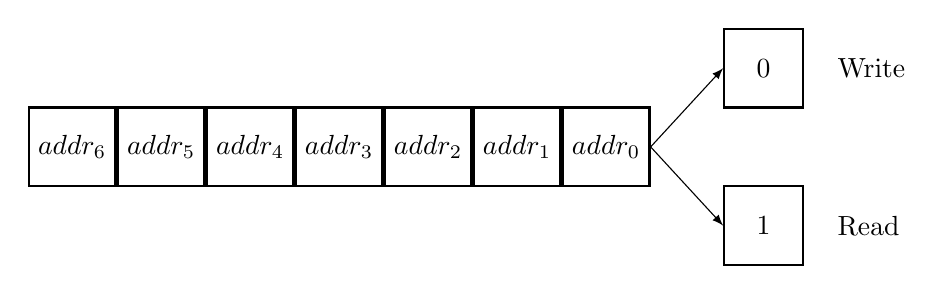
\begin{tikzpicture}
				\node (b7) at (0,0) [draw,thick,minimum width=1cm,minimum height=1cm,anchor=center] {$addr_6$};
				\node (b6) at (b7.east) [draw,thick,minimum width=1cm,minimum height=1cm,anchor=west] {$addr_5$};
				\node (b5) at (b6.east) [draw,thick,minimum width=1cm,minimum height=1cm,anchor=west] {$addr_4$};
				\node (b4) at (b5.east) [draw,thick,minimum width=1cm,minimum height=1cm,anchor=west] {$addr_3$};
				\node (b3) at (b4.east) [draw,thick,minimum width=1cm,minimum height=1cm,anchor=west] {$addr_2$};
				\node (b2) at (b3.east) [draw,thick,minimum width=1cm,minimum height=1cm,anchor=west] {$addr_1$};
				\node (b1) at (b2.east) [draw,thick,minimum width=1cm,minimum height=1cm,anchor=west] {$addr_0$};
				
				\node (bWrite) at ($(b1)+(2,1)$) [draw,thick,minimum width=1cm,minimum height=1cm,anchor=center] {0};
				\node[anchor=west] (lblWrite) at ($(bWrite.east)+(.3,0)$){Write};
				\node (bRead) at ($(b1)+(2,-1)$) [draw,thick,minimum width=1cm,minimum height=1cm,anchor=center] {1};
				\node[anchor=west] (lblRead) at ($(bRead.east)+(.3,0)$){Read};
				\draw[-latex] (b1.east) --(bWrite.west);
				\draw[-latex] (b1.east) -- (bRead.west);	
			\end{tikzpicture}
		}
	\end{frame}

	\begin{frame}
		\frametitle{Peripheral intermission - SPI}
		\textbf{S}erial \textbf{P}eripheral \textbf{I}nterface: synconous serial bus. Always in a master+multislave configuration. Has higher frequencies than $I^2C$, usually in the few tens of \si{\mega\hertz} range.
		\\\vspace{.5cm}
		\begin{center}
			\begin{adjustbox}{max width=1.5\textwidth}
				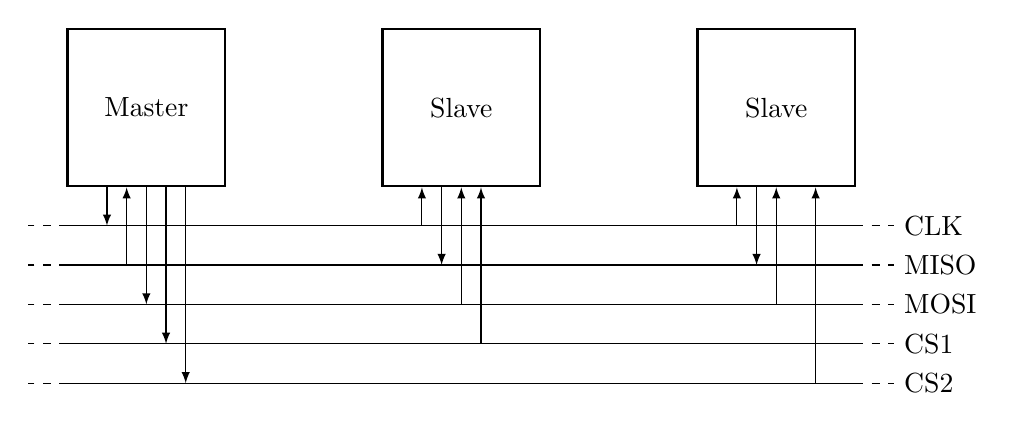
\begin{tikzpicture}
				\node (master) at (0,0) [draw,thick,minimum width=2cm,minimum height=2cm,anchor=center] {Master};
				\node (slave1) at (4,0) [draw,thick,minimum width=2cm,minimum height=2cm,anchor=center,align=center] {Slave};
				\node (slave2) at (8,0) [draw,thick,minimum width=2cm,minimum height=2cm,anchor=center] {Slave};
				\draw (-1,-1.5)coordinate (A) -- ++(10,0) (-1,-2)coordinate (B) -- ++(10,0) (-1,-2.5) coordinate(C) --++(10,0)  (-1,-3) coordinate(D) --++(10,0) (-1,-3.5) coordinate(E) --++(10,0);
				\draw [dashed] (-1,-1.5) -- ++(-.5,0) (9,-1.5) -- ++(.5,0) node[anchor=west]{CLK};
				\draw [dashed] (-1,-2) -- ++(-.5,0) (9,-2) -- ++(.5,0) node[anchor=west]{MISO};
				\draw [dashed] (-1,-2.5) -- ++(-.5,0) (9,-2.5) -- ++(.5,0) node[anchor=west]{MOSI};
				\draw [dashed] (-1,-3) -- ++(-.5,0) (9,-3) -- ++(.5,0) node[anchor=west]{CS1};
				\draw [dashed] (-1,-3.5) -- ++(-.5,0) (9,-3.5) -- ++(.5,0) node[anchor=west]{CS2};
				\draw[-latex] ($(master.south)+(-.5,0)$) coordinate (T1) -- (T1|-A); 
				\draw[latex-] ($(master.south)+(-.25,0)$) coordinate (T2) -- (T2|-B); 
				\draw[-latex] ($(master.south)+(0,0)$) coordinate (T3) -- (T3|-C);
				\draw[-latex] ($(master.south)+(.25,0)$) coordinate (T4) -- (T4|-D);
				\draw[-latex] ($(master.south)+(.5,0)$) coordinate (T5) -- (T5|-E);
				\draw[latex-] ($(slave1.south)+(-.5,0)$) coordinate (T6) -- (T6|-A); 
				\draw[-latex] ($(slave1.south)+(-.25,0)$) coordinate (T7) -- (T7|-B);
				\draw[latex-]($(slave1.south)+(0,0)$) coordinate (T8) -- (T8|-C);
				\draw[latex-] ($(slave1.south)+(.25,0)$) coordinate (T9) -- (T9|-D);
				%\draw[latex-latex] ($(slave1.south)+(.5,0)$) coordinate (T10) -- (T10|-E);	
				\draw[latex-] ($(slave2.south)+(-.5,0)$) coordinate (T11) -- (T11|-A);
				\draw[-latex] ($(slave2.south)+(-.25,0)$) coordinate (T12) -- (T12|-B);
				\draw[latex-] ($(slave2.south)+(0,0)$) coordinate (T13) -- (T13|-C);
				%\draw[latex-latex] ($(slave2.south)+(.25,0)$) coordinate (T14) -- (T14|-D);
				\draw[latex-] ($(slave2.south)+(.5,0)$) coordinate (T15) -- (T15|-E);
				\end{tikzpicture}
			\end{adjustbox}
		\end{center}
	\end{frame}

	\begin{frame}
		\frametitle{Peripheral intermission - UART}
		\textbf{U}niversal \textbf{A}syncronous \textbf{R}eceiver-\textbf{T}ransmitter: full-duples, asyncronous serial protocol. An UART connection provides point-to-point communication (NOT a bus), there is no master/slave.
		\vspace{.3cm}
		\begin{center}
			\begin{adjustbox}{max width=1.5\textwidth}
				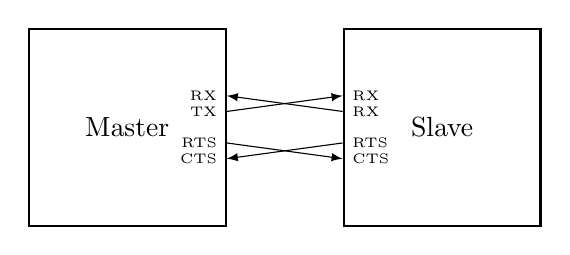
\begin{tikzpicture}
				\node (UART1) at (0,0) [draw,thick,minimum width=2.5cm,minimum height=2.5cm,anchor=center] {Master};
				\node (UART2) at (4,0) [draw,thick,minimum width=2.5cm,minimum height=2.5cm,anchor=center,align=center] {Slave};
				
				\draw[-latex] ($(UART1.east)+(0,.2)$) node[left]{\tiny TX} -- ($(UART2.west)+(0,.4)$) node[right]{\tiny RX};
				\draw[-latex] ($(UART2.west)+(0,.2)$) node[right]{\tiny RX} -- ($(UART1.east)+(0,.4)$) node[left]{\tiny RX};
				
				\draw[-latex] ($(UART1.east)+(0,-.2)$) node[left]{\tiny RTS} -- ($(UART2.west)+(0,-.4)$) node[right]{\tiny CTS};
				\draw[-latex] ($(UART2.west)+(0,-.2)$) node[right]{\tiny RTS} -- ($(UART1.east)+(0,-.4)$) node[left]{\tiny CTS};
				
				
				\end{tikzpicture}
			\end{adjustbox}
		\end{center}
	\end{frame}

	\begin{frame}
		\frametitle{Project phase - Sensors alternatives}
		There are often different sensor implementation to measure a given quantity; it is best to carry out these choices during the specifications drafting, and leave specific sensors (aka vendor) choices for this phase. Broadly speaking, it is best to take into account:
		\begin{description}
			\item[Measurement range] The measured quantity must fall inside the measurement range, possibly with a bit to spare as "guard".
			\item[Accuracy] The accuracy of the sensor must be suitable for the application. There is a thing such as too high of an accuracy, as it can weigh on the system.
			\item[ODR] Frequency of measurement is crucial to gathering the correct data. 
		\end{description}
	\end{frame}

	\begin{frame}
		\frametitle{Project phase - Memory alternatives}
		\only<1>{
			A measurement system inevitably deals with processing data, which, more often than not, must be stored as well. Microcontrollers have integrated memory chips, which sometimes can be enough. If that's not the case, additional memory must be considered, and when doing so, it is best to take into account:
			\begin{description}
				\item[Memory size] Taking into account estimated data throughput, memory requirements can be deduced.
				\item[Data permanence] Data permanence during system shutdown needs to be taken into consideration. This often translates into a technology choice for the memory.
				\item[Memory speed] Memory speed leans a little bit into the choice of technology done, but a little bit of freedom is possible even after that. As always, faster is not better for the system overall (e.g. faster means more power consumption).  
			\end{description}
		}
		\only<2>{
			\alert{Common technology choices:}
			\begin{description}
				\item[RAM] RAM is a fast, volatile memory. Adding more is done to support the already present one integrated in the microcontroller.
			\end{description}
			\begin{columns}
				\begin{column}{.3\textwidth}
					\begin{adjustbox}{max height=.3\textheight}
						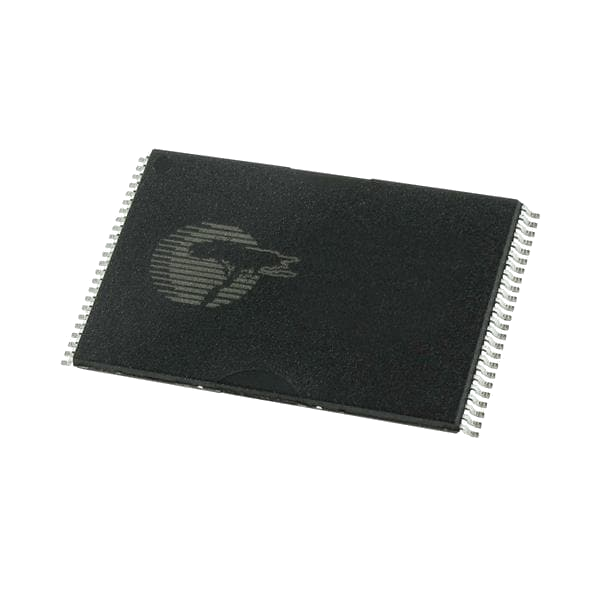
\includegraphics[width=\textwidth]{media/ram.png}
					\end{adjustbox}
				\end{column}
				\begin{column}{.7\textwidth}
					\begin{itemize}
						\item \textbf{Memory size}: for SRAM, few \si{\kilo\bit} to few \si{\mega\bit}
						\item \textbf{Data permanence}: RAM loses data after losing power
						\item \textbf{Memory speed}: SRAM are very fast, up to a point where the microcontroller is the bottleneck.
					\end{itemize}
				\end{column}
			\end{columns}
		}
		\only<3>{
			\alert{Common technology choices:}
			\begin{description}
				\item[FLASH] FLASH is a type of non volatile memory. Usually already integrated in the microcontroller in order to store the program, can be added as a separate chip in order to grant more memory capabilities. Usually is slower than RAM, has less memory size and power consumption than an SD.
			\end{description}
			\begin{columns}
				\begin{column}{.3\textwidth}
					\begin{adjustbox}{max height=.3\textheight}
						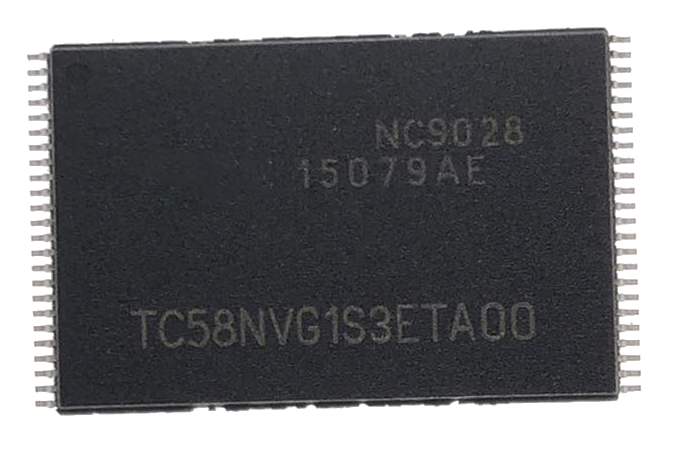
\includegraphics[width=\textwidth]{media/flash_chip.png}
					\end{adjustbox}
				\end{column}
				\begin{column}{.7\textwidth}
					\begin{itemize}
						\item \textbf{Memory size}: few \si{\kilo\bit} to few \si{\giga\bit}
						\item \textbf{Data permanence}: FLASH does not lose data without power
						\item \textbf{Memory speed}: not as fast as a RAM (few hundreds \si{\mega\hertz} clock rates at max).
					\end{itemize}
				\end{column}
			\end{columns}
		}
		\only<4>{
			\alert{Common technology choices:}
			\begin{description}
				\item[SD] SD cards are high throughput, high capacity memories. Usually added for the ease of interchanging memory support and the raw memory size.
			\end{description}
			\begin{columns}
				\begin{column}{.3\textwidth}
					\begin{adjustbox}{max height=.3\textheight}
						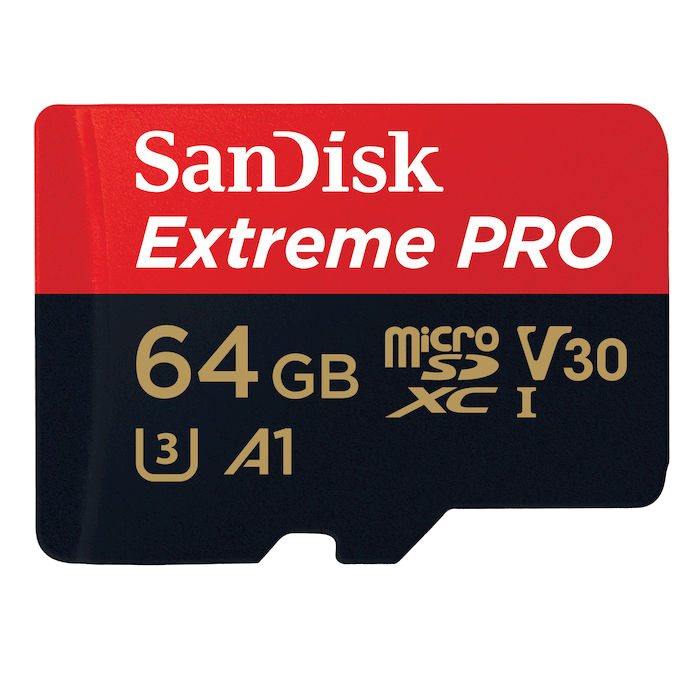
\includegraphics[width=\textwidth]{media/SD.png}
					\end{adjustbox}
				\end{column}
				\begin{column}{.7\textwidth}
					\begin{itemize}
						\item \textbf{Memory size}: hundreds of \si{\mega\bit} to hundreds of \si{\giga\bit}
						\item \textbf{Data permanence}: SD does not lose data without power
						\item \textbf{Memory speed}: SD are fast, but the real advantage is in their parallel bus (also may be a disadvantage).
					\end{itemize}
				\end{column}
			\end{columns}
		}
	\end{frame}

	\begin{frame}
		\frametitle{Project phase - Communication alternatives}
		\only<1>{
			Sometimes seen as an alternative to storing data, transmitting data outside the system can be quite a central part of the overall functionality. Data transmission can be either via wire or wireless. In the case of wireless transmission, the most important characteristics to consider are:
			\begin{description}
				\item [Range] Radio transmission is range limited, especially when considering a constraint-heavy embedded system. This will mostly impact the technology choice.
				\item [Throughput] Similarly to memory size requirements, the data quantity that the system wishes to transmit has a big impact in the choice of technology.
				\item [Power consumption] Different technologies offer very different power consumptions.
			\end{description}	
		}
		\only<2>{
			\alert{Common technology choices:}
			\begin{description}
				\item[BT] Bluetooth is a short range radio protocol. Its classic implementation offers a good throughput for streaming data (data throughput $\sim$\SI{2}{\mega\bit\per\second}); its low energy implementation offers a much lower throughput for quite a big improvement on the energy consumption side.
			\end{description}
			\begin{columns}
				\begin{column}{.3\textwidth}
					\begin{adjustbox}{max height=.3\textheight}
						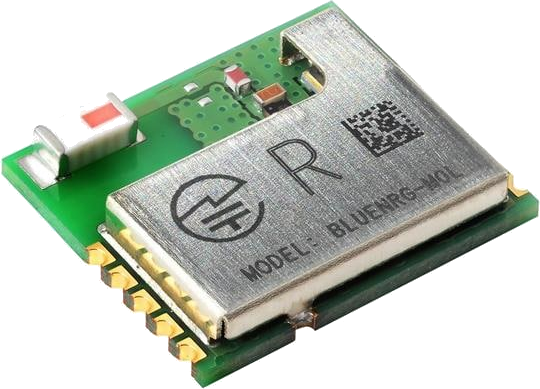
\includegraphics[width=\textwidth]{media/BT.png}
					\end{adjustbox}
				\end{column}
				\begin{column}{.7\textwidth}
					\begin{itemize}
						\item \textbf{Range}: \SIrange{10}{30}{\meter} for BT classic, few meters for BLE.
						\item \textbf{Throughput}: up to $\sim$\SI{2}{\mega\bit\per\second} BT classic, $\sim$\SI{100}{\kilo\bit\per\second} BLE.
						\item \textbf{Power consumption}: $\sim$\SI{100}{\milli\watt} BT classic, tens of \si{\milli\watt} BLE.
					\end{itemize}
				\end{column}
			\end{columns}
		}
		\only<3>{
			\alert{Common technology choices:}
			\begin{description}
				\item[WiFi] WiFi is a medium range radio protocol. It offers a very high throughput at the cost of high power consumption	
			\end{description}
			\begin{columns}
				\begin{column}{.3\textwidth}
					\begin{adjustbox}{max height=.3\textheight}
						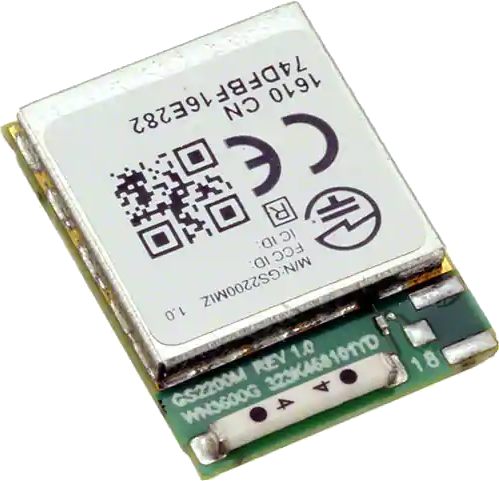
\includegraphics[width=\textwidth]{media/wifi.png}
					\end{adjustbox}
				\end{column}
				\begin{column}{.7\textwidth}
					\begin{itemize}
						\item \textbf{Range}: tens of meters (unimpeded)
						\item \textbf{Throughput}: theoretical max of \SI{500}{\mega\bit\per\second}
						\item \textbf{Power consumption}: up to \SI{500}{\milli\watt}.
					\end{itemize}
				\end{column}
			\end{columns}
		}
		\only<4>{
			\alert{Common technology choices:}
			\begin{description}
				\item[LoRa] LoRa is a long range radio protocol for low throughput, low power consumption communication. It uses sub-GHz frequency ranges.
			\end{description}
			\begin{columns}
				\begin{column}{.3\textwidth}
					\begin{adjustbox}{max height=.3\textheight}
						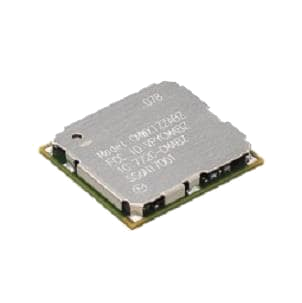
\includegraphics[width=\textwidth]{media/lora.png}
					\end{adjustbox}
				\end{column}
				\begin{column}{.7\textwidth}
					\begin{itemize}
						\item \textbf{Range}: up to \SI{10}{\kilo\meter} if unimpeded.
						\item \textbf{Throughput}: few \si{\kilo\bit\per\second}
						\item \textbf{Power consumption}: \SIrange{100}{200}{\milli\watt}.
					\end{itemize}
				\end{column}
			\end{columns}
		}
		\only<5>{
			\alert{Common technology choices:}
			\begin{description}
				\item[sub-GHz] If customization is needed, a sub-GHz radio can be employed. A custom protocol needs to be defined on top of it.
			\end{description}
			\begin{columns}
				\begin{column}{.3\textwidth}
					\begin{adjustbox}{max height=.3\textheight}
						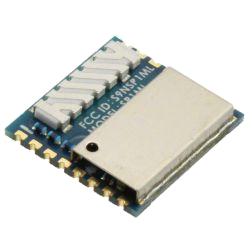
\includegraphics[width=\textwidth]{media/subGhz.png}
					\end{adjustbox}
				\end{column}
				\begin{column}{.7\textwidth}
					\begin{itemize}
						\item \textbf{Range}: application dependant
						\item \textbf{Throughput}: application dependant
						\item \textbf{Power consumption}: application dependant
					\end{itemize}
				\end{column}
			\end{columns}
		}
	\end{frame}

	\begin{frame}
		\frametitle{Antennas intermission - Types}
		After choosing the desired technology, there usually is another issue to address:
		\begin{itemize}
			\item Use a RF module, a complete integrated system w/ antenna: bigger, more expensive but easy to integrate
			\item Use a SoC that requires an external antenna: difficult to design correctly, high initial cost but cheaper afterwards
		\end{itemize}
		\begin{columns}[T]
			\begin{column}{.25\textwidth}
				\centering\textbf{Ceramic antenna}\\
				\begin{adjustbox}{max height=.3\textheight,max width=.9\textwidth}
					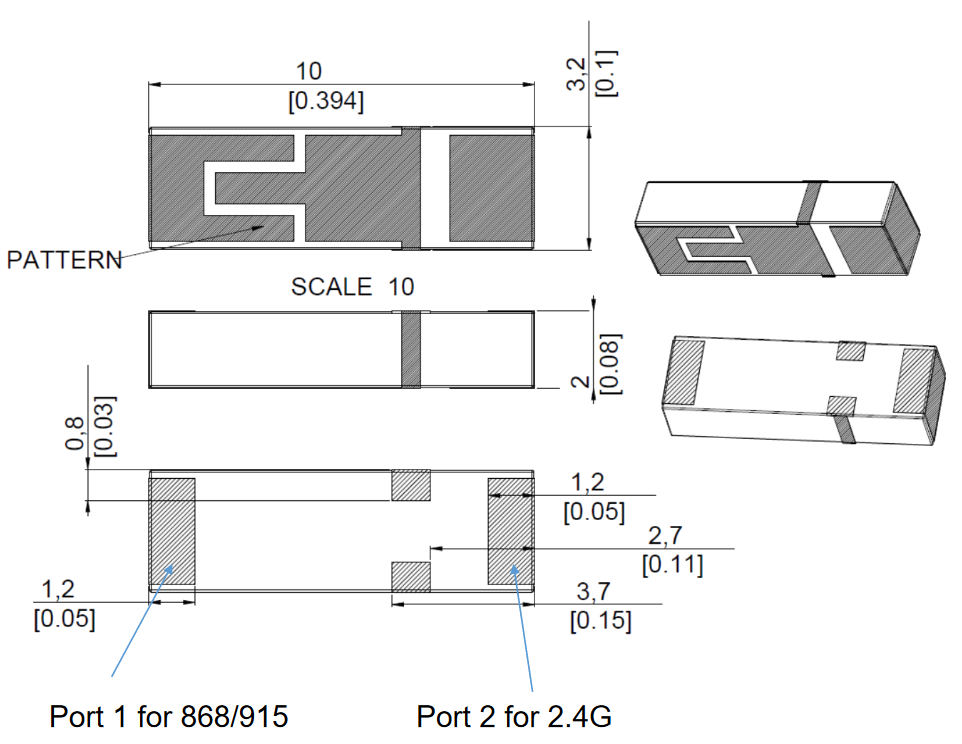
\includegraphics{media/ceramic_ant.PNG}
				\end{adjustbox}
			\end{column}
			\begin{column}{.25\textwidth}
				\centering\textbf{Patch antenna}\\
				\begin{adjustbox}{max height=.3\textheight,max width=.9\textwidth}
					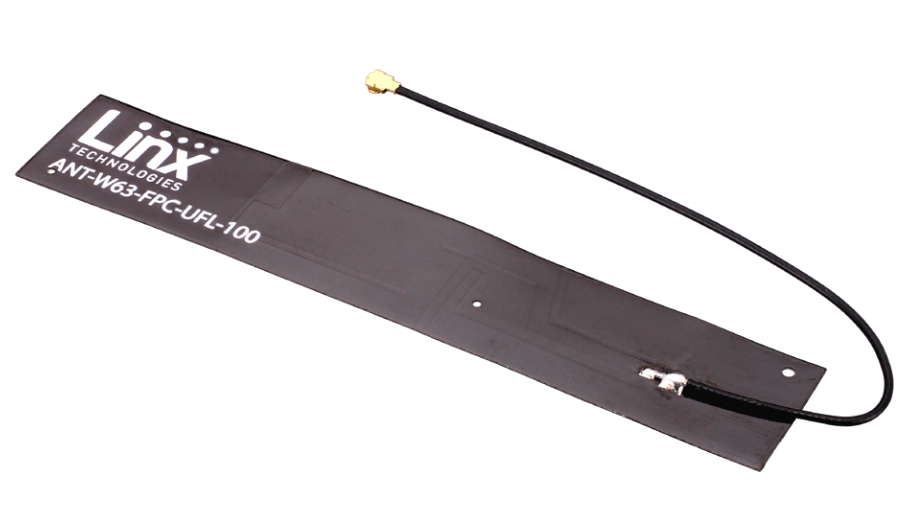
\includegraphics{media/patch_ant.PNG}
				\end{adjustbox}
			\end{column}
			\begin{column}{.25\textwidth}
				\centering\textbf{Stick antenna}\\
				\begin{adjustbox}{max height=.3\textheight,max width=.9\textwidth}
					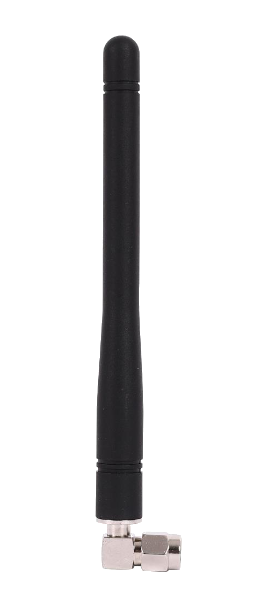
\includegraphics{media/stick_ant.PNG}
				\end{adjustbox}
			\end{column}
			\begin{column}{.25\textwidth}
				\centering\textbf{Trace antenna}\\
				\begin{adjustbox}{max height=.3\textheight,max width=.9\textwidth}
					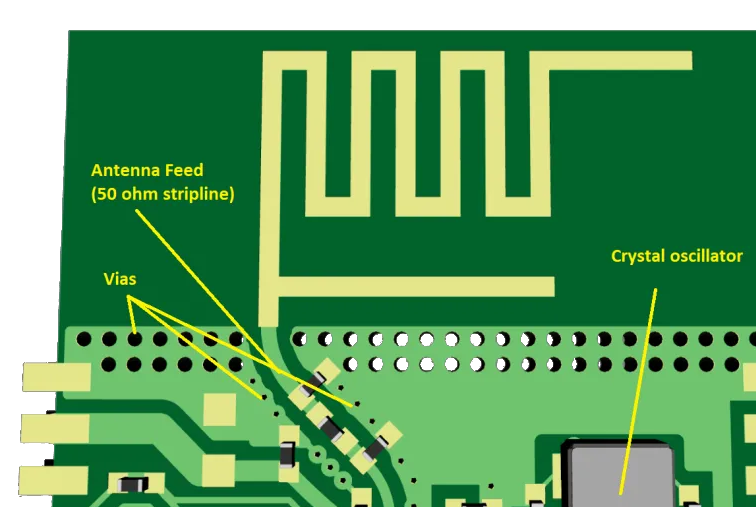
\includegraphics{media/trace_ant.PNG}
				\end{adjustbox}
			\end{column}
		\end{columns}
	\end{frame}

	\begin{frame}
		\frametitle{Antennas intermission - Lobes}
		When choosing an antenna, careful consideration should go towards the lobes. They provide a measure of the antenna \textbf{gain} and \textbf{directionality}.
		\begin{center}
			\begin{adjustbox}{max width=.95\textwidth,max height=.7\textheight}	
				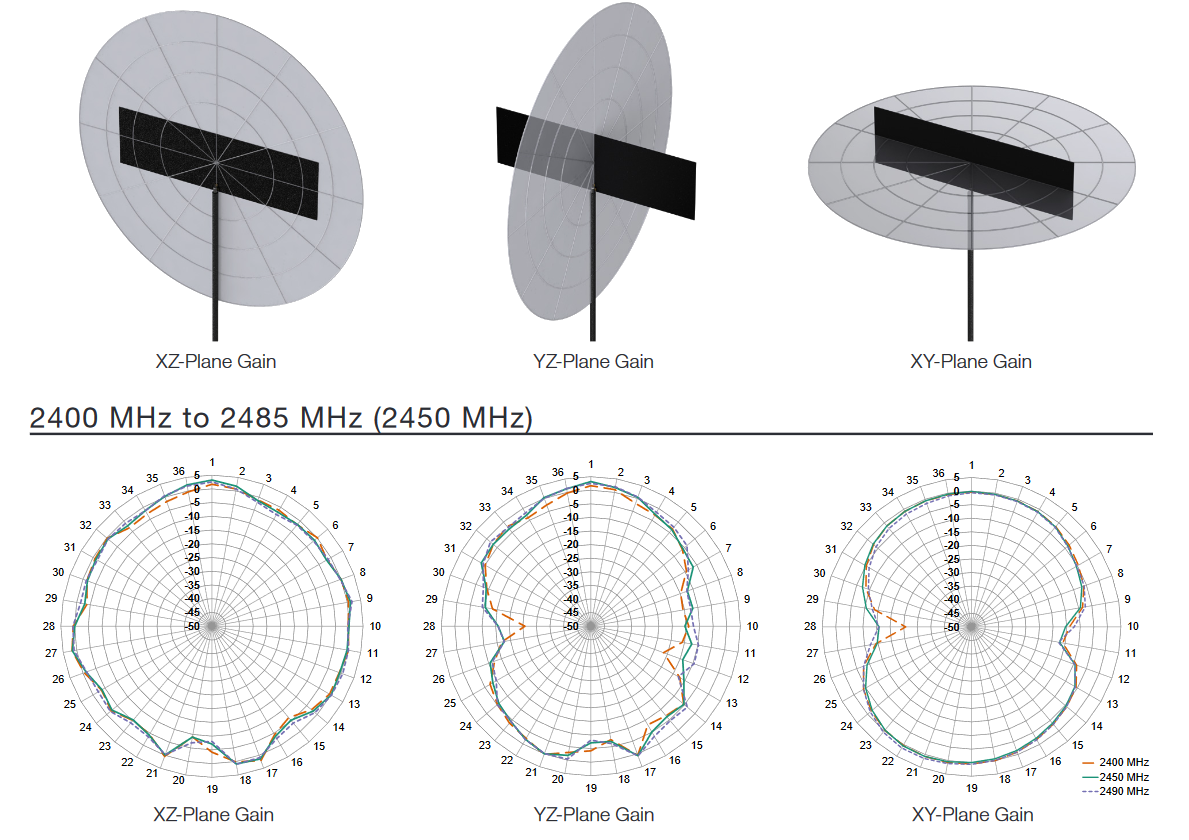
\includegraphics{media/ant_lobes.png}
			\end{adjustbox}
		\end{center}
	\end{frame}

	\begin{frame}
		\frametitle{Project phase - System support and additional functionalities}
		There are \textbf{others system blocks} that need to be defined in order to complete the project; notably a power block, responsible of providing the supply rails to all the system components, and various connectors needed to support some of the system functionalities. Other blocks can be optionally considered, if needed by the application, such as:
		\begin{itemize}
			\item A \textbf{RTC}, useful to keep a stable time reference even when employing a low power-state of other system blocks.
			\item \textbf{Gas-gauge ICs}, to keep the battery charge state controlled.
			\item \textbf{Battery charging ICs}, to regulate the current when charging the battery (if applicable).
			\item \textbf{Multiplexers}, to make use of a lower number of microcontroller pins to drive or read multiple I/Os.
		\end{itemize}
	\end{frame}

	\begin{frame}
		\frametitle{Project phase - Batteries}
		\only<1>{
			There are a lot of cells chemistries, but the focus for embedded systems is towards \textbf{lithium-ion rechargeable batteries}, for their high energy density and affordable cost. A single lithium-ion cell has a voltage ranging from $\sim$\SI{2.5}{\volt} at \SI{0}{\percent} SoC, to $\sim$\SI{4.2}{\volt} at \SI{100}{\percent} SoC, so voltage regulation is needed. Recharging the battery also requires a dedicated IC.\\
			When choosing a battery, look out for:
			\begin{description}
				\item[Capacity] Often expressed in \si{\milli\ampere\hour}, it is a measure of the maximum energy stored in the battery. A value of \SI{300}{\milli\ampere\hour} means that the battery will be drained completely if discharged with a constant \SI{300}{\milli\ampere} current for \SI{1}{\hour}.
				\item[Temperature range] Battery chemistry performance is strictly related to the temperature of the battery itself; choose a battery that suits the application (outdoor, indoor, ...) 
			\end{description} 
		}
	\only<2>{
		Lithium-ion rechargeable batteries are very widespread in embedded systems given that they have useful characteristics for these applications:\\
		\begin{columns}
			\begin{column}{.6\textwidth}
				\begin{itemize}
					\item High energy density $\sim$\SI{200}{\watt\hour\per\kilo\gram}
					\item Low discharge memory
					\item Low self-discharge current
				\end{itemize} 
			\end{column}
			\begin{column}{.4\textwidth}
				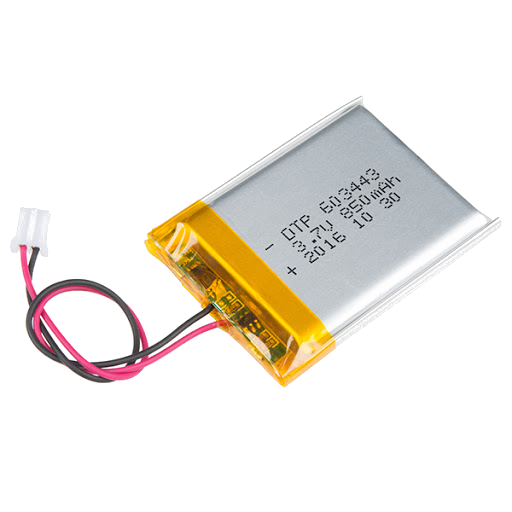
\includegraphics[width=.6\textwidth]{media/battery.png}
			\end{column}
		\end{columns}
		
	}
		 
	\end{frame}

	\begin{frame}
		\frametitle{Project phase - System voltage regulators}
		\only<1>{
			All system functionalities rely on the actual blocks being correctly powered; more often than not, systems require more than one supply rail to function in an efficient manner. A good design choice could be to allow for (if possible) two supplies: 
			\begin{itemize}
				\item A main, non controllable supply that is present as soon as a battery (or other form of external power) is connected. All core functionalities of the system can be powered under this supply (i.e. microcontroller and core sensors).
				\item An ancillary, controllable supply; this secondary supply can be controlled by the MCU, with the goal of managing power more efficiently in the system.
			\end{itemize}
		}
		\only<2-3>{
			These supplies are normally generated by DC-DC converters; the choice for a voltage regulator usually comes down to \\
			\vspace{.3cm}
			\begin{columns}[T]
				\begin{column}{.5\textwidth}
					\centering \textbf{Linear regulators}\\\vspace{.1cm}
					\only<2>{
						\begin{adjustbox}{max width=\textwidth}
							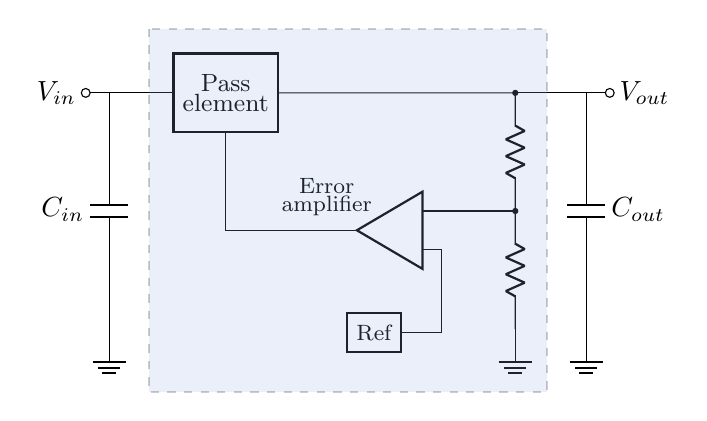
\begin{tikzpicture}
								\node [draw,thick,minimum width=1cm,minimum height=1cm,align=center,execute at begin node=\setlength{\baselineskip}{3pt}] (pass) at(0,0){\small Pass\\\small element};
								\draw (pass.east) -- ++(3,0) coordinate(out) to[R,*-*,/tikz/circuitikz/bipoles/length=.8cm] ++ (0,-1.5) coordinate(fb) to [R,/tikz/circuitikz/bipoles/length=.8cm] ++(0,-1.5) to node[ground]{} ++(0,0) coordinate(end);
								\node [plain amp,xscale=-.5,yscale=.5,anchor=in up](err) at($(fb)+(-1,0)$){};
								\node [align=center,execute at begin node=\setlength{\baselineskip}{3pt}] (lblErr) at ($(err)+(-.8,.42)$){\footnotesize Error\\\footnotesize amplifier};
								\draw (err.out) -| (pass.south) (fb) -- (err.in up);
								\node [draw,thick,minimum width=.5cm,minimum height=.5cm] (bgr) at ($(err)+(-.2,-1.3)$){\footnotesize Ref};
								\draw (bgr.east) -- ++(.5,0) |- (err.in down);
								\draw (pass.west) -- ++(-.8,0)coordinate(in) to [C,l_=$C_{in}$,/tikz/circuitikz/bipoles/length=.8cm] ++(0,-3) to node[ground]{}++(0,0) (out) -- ++(.9,0) coordinate(out1) to [C,l=$C_{out}$,/tikz/circuitikz/bipoles/length=.8cm] ++(0,-3) to node[ground]{}++(0,0);
								\draw (in) to[short,-o] ++(-.3,0) node[left]{$V_{in}$} (out1)  to[short,-o] ++(.3,0) node[right]{$V_{out}$};
								\draw [thick, dashed, fill=uniBGLightBlue,opacity=.2] ($(pass.north west)+(-.3,.3)$) rectangle ($(end)+(.4,-.8)$);
							\end{tikzpicture}
						\end{adjustbox}
					}
					\only<3>{
						\begin{itemize}
							\item[\cmark] Low output noise
							\item[\cmark] Simple and low cost
							\item[\cmark] Fast transient response
							\item[\xmark] Low efficiency
							\item[\xmark] Thermal problems
						\end{itemize}
					}
					
				\end{column}
				\begin{column}{.5\textwidth}
					\centering \textbf{Switching regulators}\\\vspace{.1cm}
					\only<2>{
						\begin{adjustbox}{max width=\textwidth}
							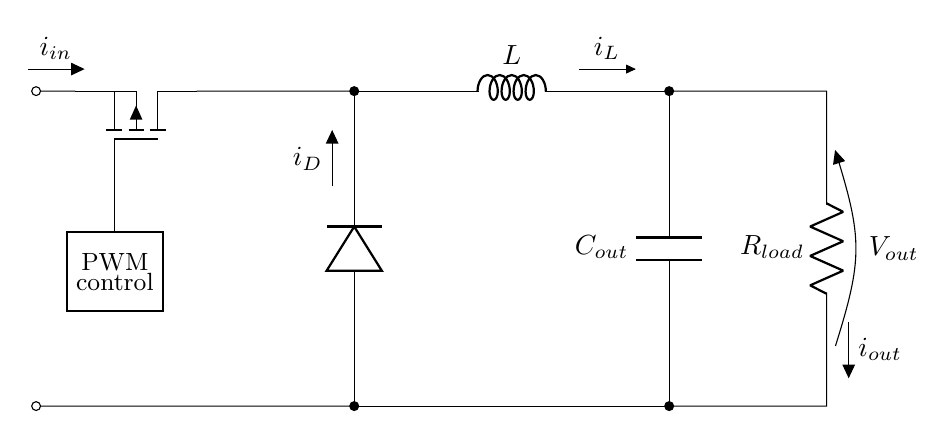
\begin{tikzpicture}[voltage dir=old]
								\node[pigfete,rotate=90](mos) at (0,0){};
								\draw ($(mos.D)+(2,0)$) to [L,l=$L$,f=$i_L$, current arrow scale=24] ++(4,0) coordinate(out) to[C,l_=$C_{out}$] ++(0,-4) coordinate(outgnd) to[short,*-*]++(-4,0) coordinate(ingnd) to[empty diode,f=$i_D$] ($(mos.D)+(2,0)$);
								\draw (mos.D) to[short,-*]($(mos.D)+(2,0)$) (mos.S) to[black,short,-o,f<_=$i_{in}$] ++(-.5,0) coordinate(in) (ingnd) to[short,-o] (ingnd-|in) (out) to[short,*-] ++(2,0) to[R,l_=$R_{load}$,f=$i_{out}$, v^=$V_{out}$] ++(0,-4) |-(outgnd);
								\node [draw,thick,minimum width=1cm,minimum height=1cm,anchor=north,align=center,execute at begin node=\setlength{\baselineskip}{3pt}] (CTRL) at ($(mos.G)+(0,-.8)$){\small PWM\\\small control};
								\draw (mos.G) -- (CTRL.north);
							\end{tikzpicture}
						\end{adjustbox}
					}
					\only<3>{
						\begin{itemize}
							\item[\cmark] High efficiency
							\item[\cmark] High output currents
							\item[\cmark] No thermal problems
							\item[\xmark] Output ripple noise and EMI
							\item[\xmark] Expensive and requires external components
						\end{itemize}
					}
					
				\end{column}
			\end{columns}	
		}	
	\end{frame}



	\begin{frame}
		\frametitle{Development phase - Outline}
		\textbf{Goal:} develop hardware and firmware to create system functionalities.
		\begin{itemize}
			\item PCB development\begin{itemize}
				\item Schematic drawing
				\item Layout drawing
			\end{itemize}
			\item Firmware development\begin{itemize}
				\item Hardware and firmware link
				\item FSM definition and implementation
				\item Event-driven firmware development
			\end{itemize}
		\end{itemize}
	\end{frame}

	\begin{frame}
		\frametitle{Development phase - PCB introduction}
		\textbf{P}rinted \textbf{C}ircuit \textbf{B}oards are, as the name suggest, \textbf{circuits printed onto a mechanical support}. A PCB is essentially a collection of metal layers (interconnections) laminated between a non-conductive support (usually fiberglass weave); it is manufactured starting from the inner layers etching away unwanted metal areas. More layers are then added (2 at a time, top and bottom) to this "sandwich" and the process is repeated until the PCB is complete.\\
		\begin{center}
			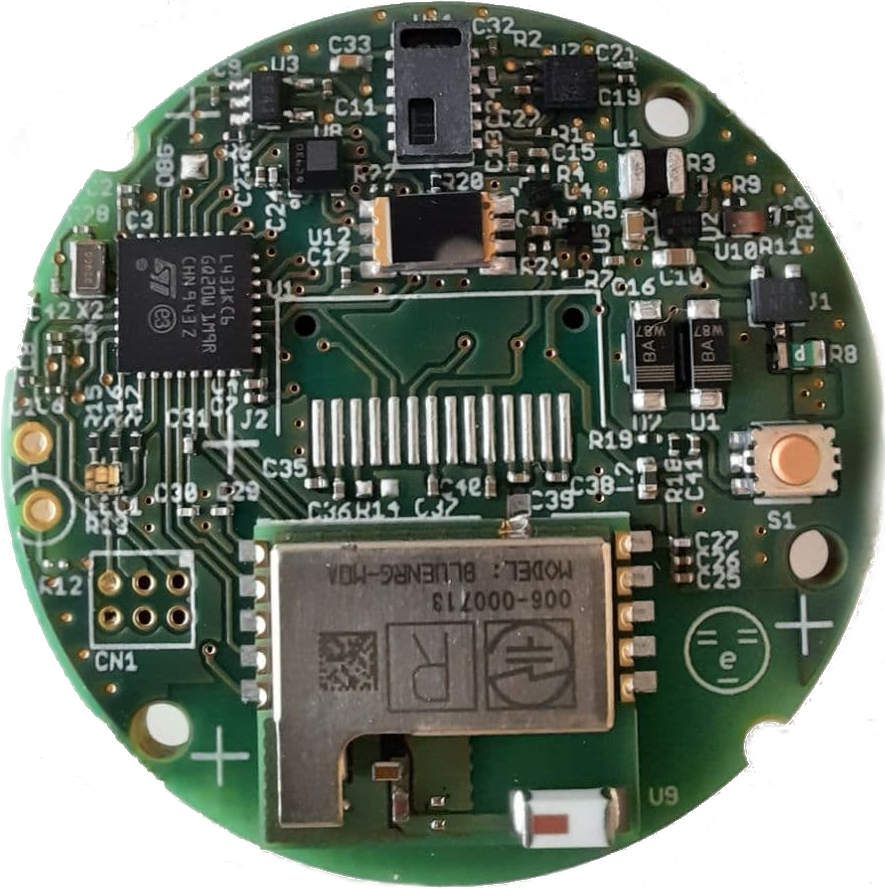
\includegraphics[width=.2\paperwidth]{media/board.png}
		\end{center}
	\end{frame}


	\begin{frame}
		\frametitle{Development phase - PBC introduction}
		A PCB can be manufactured with 3 elements:
		\begin{columns}[t]
			\begin{column}{0.33\paperwidth}
				\begin{itemize}
					\item Stackup
				\end{itemize}
				\centering
				\vspace{.2cm}
				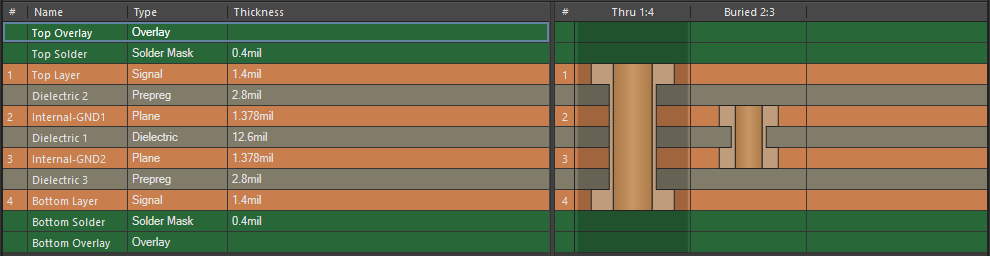
\includegraphics[width=.75\textwidth]{media/Stackup.png}
			\end{column}
			\begin{column}{0.33\paperwidth}
				\begin{itemize}
					\item Gerbers
				\end{itemize}
				\centering
				\vspace{.2cm}
				\begin{adjustbox}{max height=.35\textheight}
					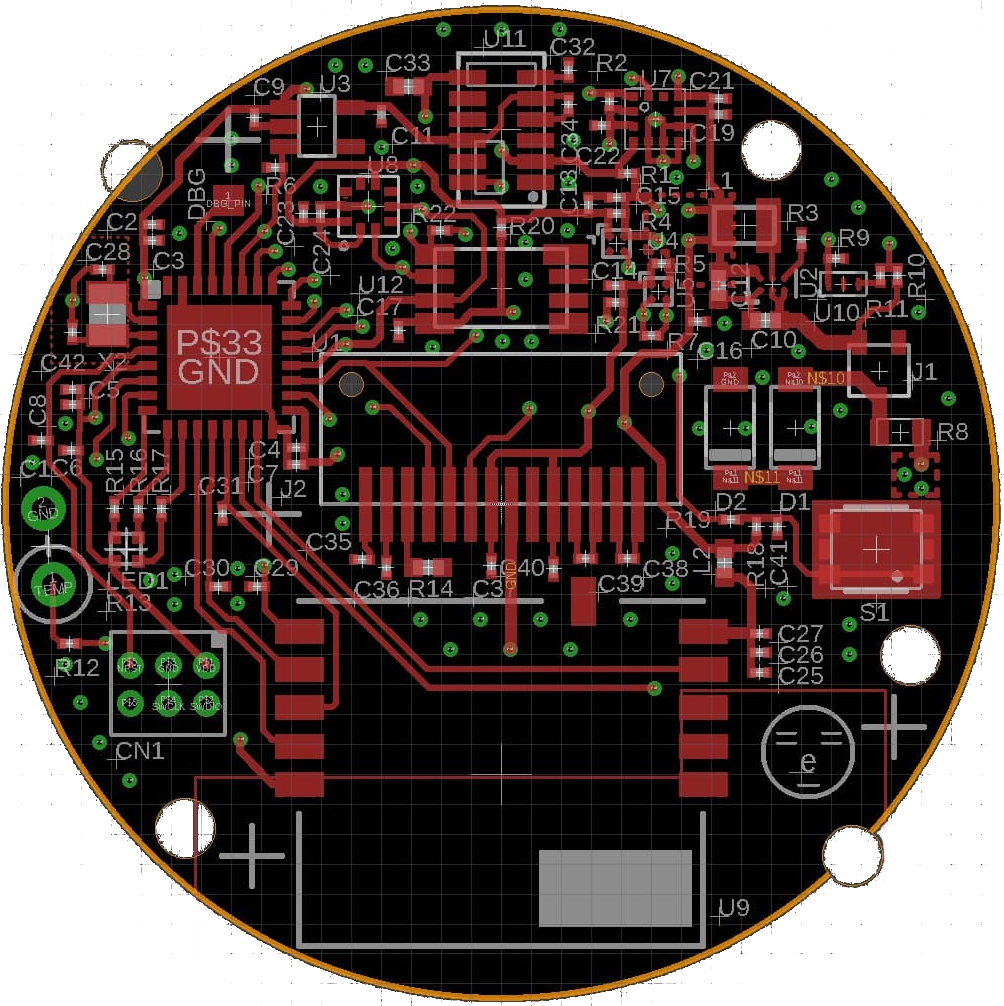
\includegraphics{media/gerbers.png}
				\end{adjustbox}
				
			\end{column}
			\begin{column}{0.33\paperwidth}
				\begin{itemize}
					\item Bill of material
				\end{itemize}
				\centering
				\vspace{.2cm}
				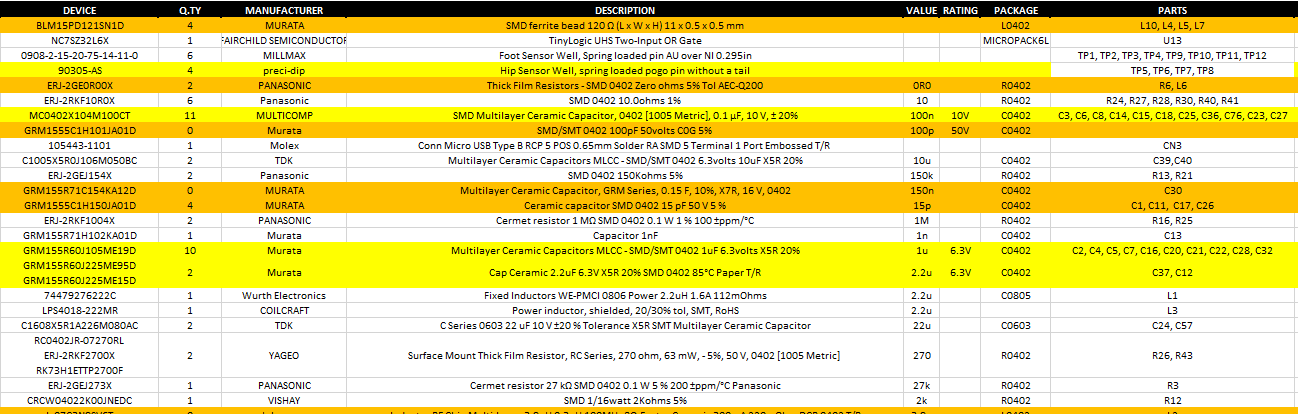
\includegraphics[width=.75\textwidth]{media/BOM.png}
			\end{column}
		\end{columns}
	\end{frame}

	\begin{frame}
		\frametitle{Development phase - PCB schematic}
		\only<1>{
			The \textbf{PCB schematic} is an \textbf{abstracted view of the interconnections} in the system. All selected components are placed as abstract blocks and connected properly in this view; some connections can be modified iteratively if a different choice eases the layout process.
			\vspace{-1cm}
			\begin{center}
				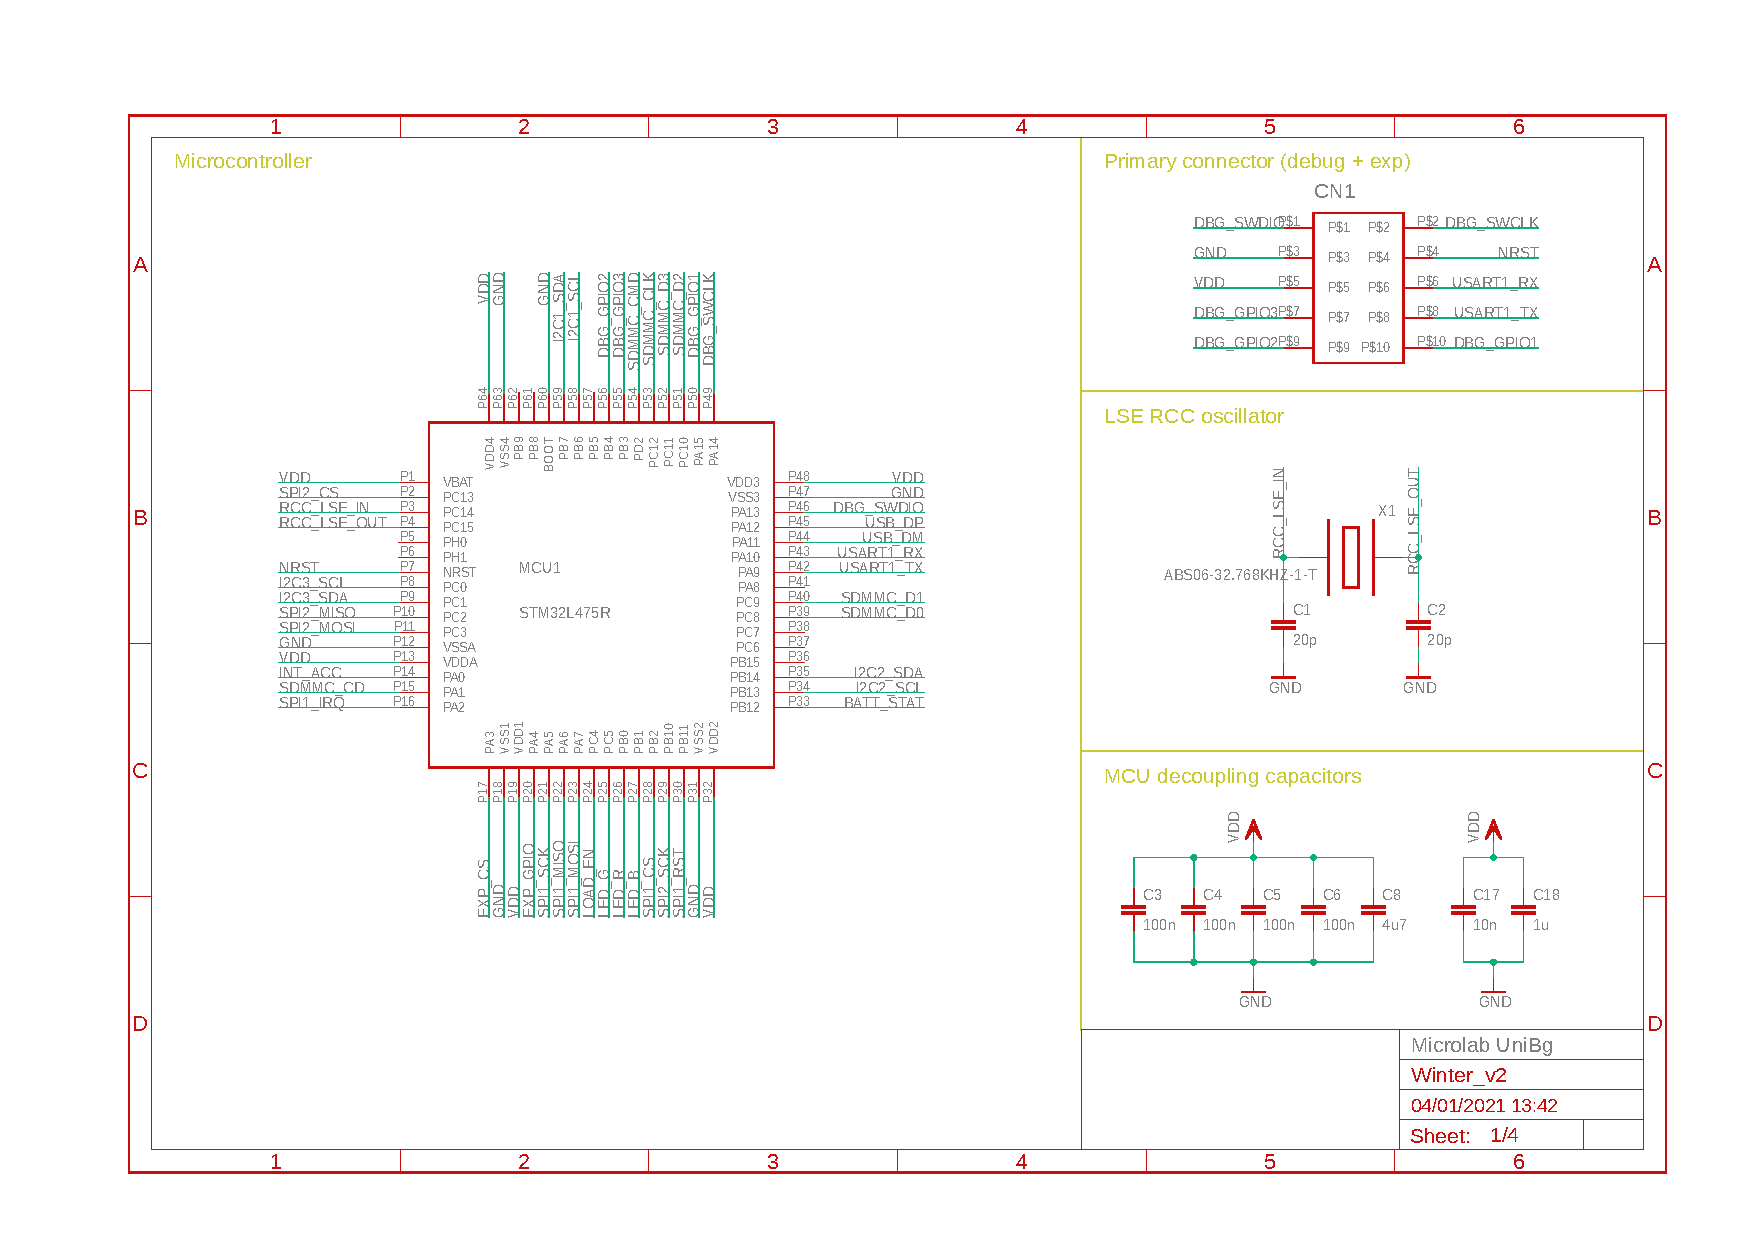
\includegraphics[width=.55\textwidth]{media/schematic.pdf}
			\end{center} 
		}
	\only<2>{
		Once the schematic is drawn, an \textbf{E}lectrical \textbf{R}ule \textbf{C}heck is performed, to lower the possibility of errors in the design. Some examples of errors reported by the ERC:
		\begin{itemize}
			\item floating input pins;
			\item nets with multiple names;
			\item power pins unconnected;
			\item nets with only one pin;
			\item ...
		\end{itemize}
	}
	\end{frame}

	\begin{frame}
		\frametitle{Schematic design intermission - Footprints}
		When adding a component to a schematic, it must be linked to a symbol and to a footprint. Although the former is useful to have drawn nicely, the latter is of the utmost importance. A footprint represents the interconnection between a PCB and a IC and must be realized to specification.\\\vspace{.5cm}
		\begin{columns}
			\begin{column}{.5\textwidth}
				\centering
				\begin{adjustbox}{max height=.5\textheight}
					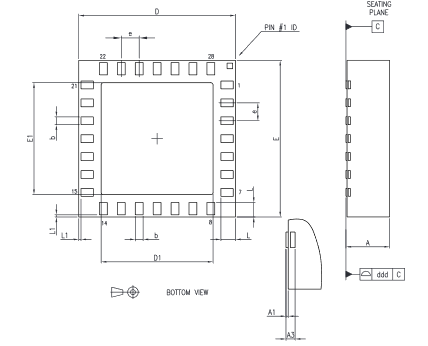
\includegraphics[width=\textwidth]{media/footprint_data.png}
				\end{adjustbox}
			\end{column}
			\begin{column}{.5\textwidth}
				\centering
				\begin{adjustbox}{max height=.5\textheight}
					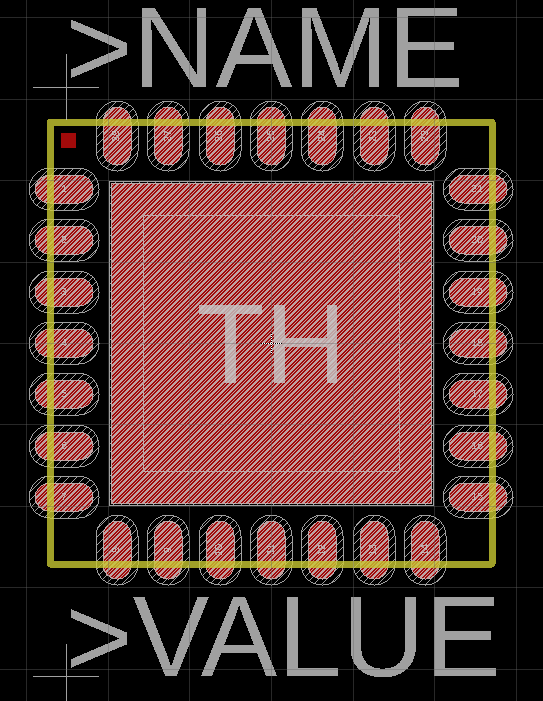
\includegraphics[width=\textwidth]{media/footprint_drawn.png}
				\end{adjustbox}
			\end{column}
		\end{columns}
	\end{frame}
		

	\begin{frame}
		\frametitle{Development phase - PCB layout}
		\only<1>{
			The PCB layout is the \textbf{implementation of the connections} drawn in the schematic. All selected components are placed and represented as they actually will be on the final PCB; all proportions in the layout are what will be present on the manufactured PCB. The layout is actually realized by \textbf{tracing} (drawing) the \textbf{interconnections}, guided by the layout tool; the tool uses information from the schematic to guide the process.
			\begin{center}
				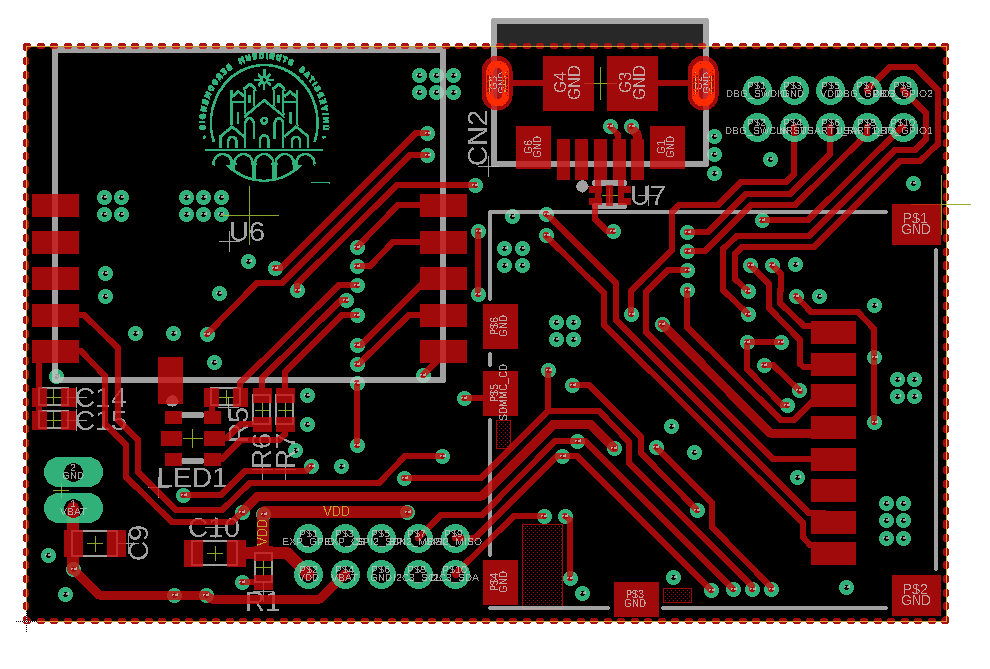
\includegraphics[width=.35\textwidth]{media/layout.png}
			\end{center} 
		}
		\only<2>{
			Once the layout is drawn, an \textbf{D}esign \textbf{R}ule \textbf{C}heck is performed, ensure that the design can be fabricated. Some examples of errors reported by the DRC:
			\begin{itemize}
				\item holes too smalls;
				\item routes too small;
				\item gaps between routes too small;
				\item components too close to each other or to the PCB border;
				\item ...
			\end{itemize}
		}
	\end{frame}

	\begin{frame}
		\frametitle{Layout design intermission - Placement}
		\only<1>{
			Component placement refers to the process of arranging the components onto the board. It is done before starting to trace the routes with the goal of:
			\begin{itemize}
				\item \textbf{verifying that all components fit} nicely inside the defined board shape/dimensions
				\item creating (physical) \textbf{separation between analog and digital} components
				\item finding out best position and orientation to \textbf{minimize trace length and complexity}
				\item \textbf{identifying pin alternatives} that can lead to better layouts
			\end{itemize}
		}
	\only<2>{
		\begin{columns}
			\begin{column}{.5\textwidth}
				\begin{adjustbox}{max height=.8\textheight}
					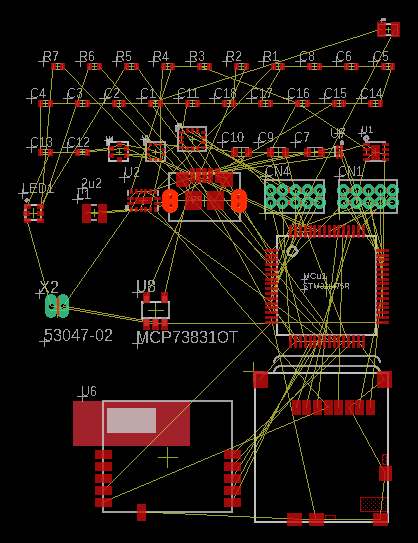
\includegraphics[width=\textwidth]{media/pre_placement.png}
				\end{adjustbox}	
			\end{column}
			\begin{column}{.5\textwidth}
				\begin{adjustbox}{max height=.8\textheight}
					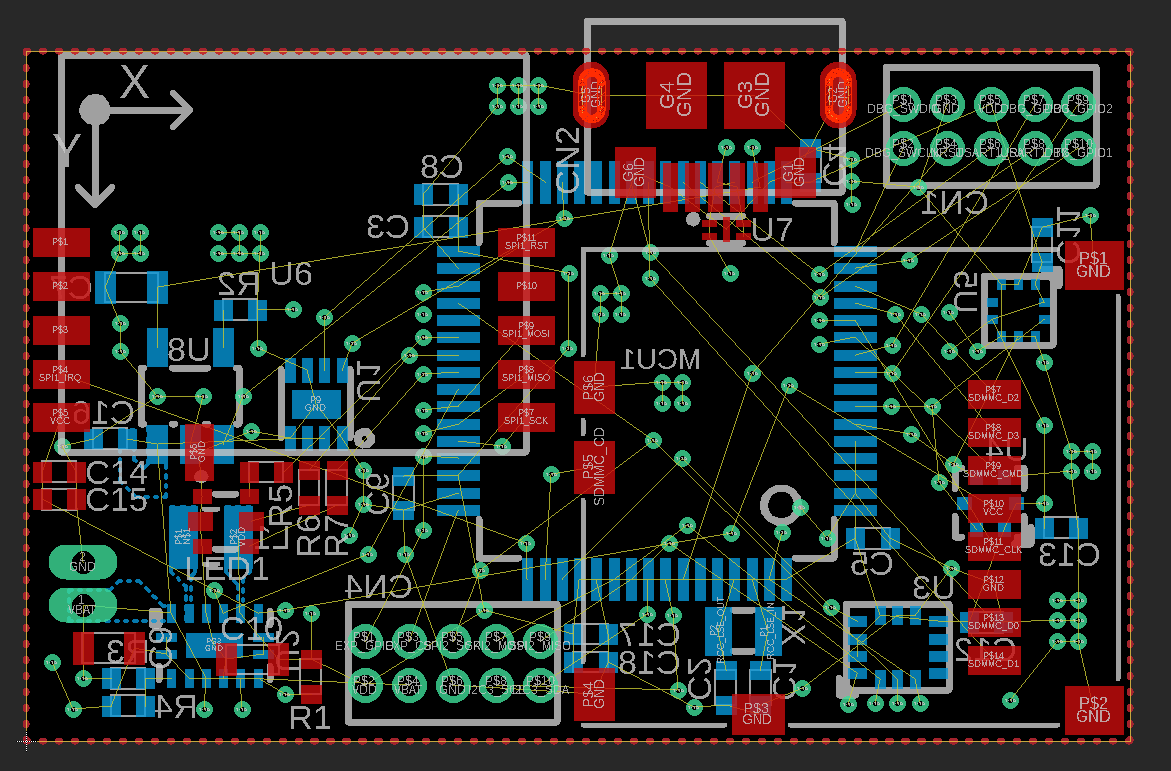
\includegraphics[width=\textwidth]{media/post_placement.png}
				\end{adjustbox}
			\end{column}
		\end{columns}
	}	
	\end{frame}

	\begin{frame}
		\frametitle{Layout design intermission - Routing}
		Routing is a process that can be easy to approach, but difficult to master, Some guidelines to keep in mind when routing:
		\begin{itemize}
			\item keep traces short \& direct
			\item Always have a ground plane
			\item Keep the ground plane as uninterrupted as possible and route high frequency traces "on top" of the ground plane
			\item Try to avoid 90° turns on traces
			\item Size traces according to current; rule of thumb 10 mils $\simeq$ \SI{0.3}{A}.
		\end{itemize}
	\end{frame}

	\begin{frame}
		\frametitle{Development phase - Hardware and firmware link}
		It is necessary to \textbf{define all the interfaces between} the already designed \textbf{PCB and the firmware} as a first step of its development. The microcontroller is the bridge between the hardware and the firmware, it must be configured.\\
		Configuration can happen by simpling writing code that configures the microcontroller on startup, OR by using tools to generate this configuration code; this process will define:
		\begin{itemize}
			\item Pin configuration
			\item Internal peripherals settings
			\item Clock tree
		\end{itemize}
	\end{frame}

	\begin{frame}
		\frametitle{Development phase - Pin configuration}
		Microcontroller pin functions must be defined; using a tool to do so simply means assigning a function to each pin (remember that communication peripherals require more than one pin!).\\
		\begin{center}
			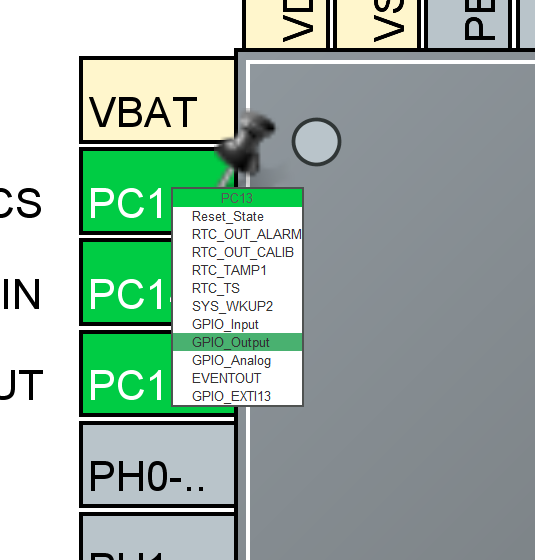
\includegraphics[width=.3\textwidth]{media/pin_config.png}
		\end{center}
	\end{frame}

	\begin{frame}
		\frametitle{Development phase - GPIOs}
		Most of the microcontroller pins can be set as \textbf{G}eneral \textbf{P}urpose \textbf{I}nput \textbf{O}utput (GPIO), which are a part of the microcontroller interface toward the extern (PCB). They must be set to a specific function:
		\begin{itemize}
			\item input
			\item output
			\item interrupt
		\end{itemize}
		The internal circuitry of the GPIO can also be set:
		\begin{itemize}
			\item pull-up/pull-down
			\item open-drain/push-pull
		\end{itemize}
	\end{frame}

	\begin{frame}
		\frametitle{Development phase - GPIOs}
		Function-based GPIO classification:
		\vspace{.3cm}
		\begin{columns}[T]
			\begin{column}{.27\textwidth}
				\textbf{Output}\\
				Digital output; can be either high (1) or low (0). Cannot source much current (\SIrange{15}{20}{\milli\ampere} max)
			\end{column}
			\begin{column}{.27\textwidth}
				\textbf{Input}\\
				Digital input; can read either high (1) or low (0). High input impedance.
			\end{column}
			\begin{column}{.27\textwidth}
				\textbf{Interrupt}\\
				Digital input, but edge triggered (configurable). An edge on this pin creates a block of current code execution to allow a specific response.
			\end{column}
		\end{columns}
	\end{frame}
	
	\begin{frame}
		\frametitle{Development phase - GPIOs}
		Internal circuit classification:
		\vspace{.3cm}
		\begin{columns}[T]
			\begin{column}{.5\textwidth}
				\centering
				\textbf{Pull-up}\\\vspace{.5cm}
				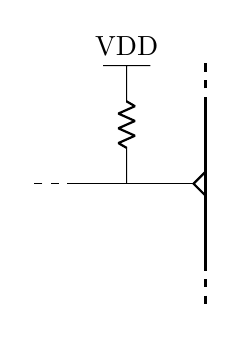
\begin{tikzpicture}
					\draw [very thick] (0,1) -- ++(0,-2);
					\draw [very thick, dashed] (0,1) -- ++(0,.6) (0,-1) -- ++(0,-.6);
					\draw [thick] (0,.15) -- ++(-.15,-.15) -- ++(.15,-.15);
					\draw (-.15,0) -- ++(-1.5,0) coordinate (i);
					\draw (-1,0) to[R,/tikz/circuitikz/bipoles/length=20pt] ++(0,1.5) node[above]{VDD} -- ++(-.3,0) --++(.6,0);
					\draw [dashed] (i) -- ++(-.6,0);
				\end{tikzpicture}
			\end{column}
			\begin{column}{.5\textwidth}
				\centering
				\textbf{Pull-down}\\\vspace{.5cm}
				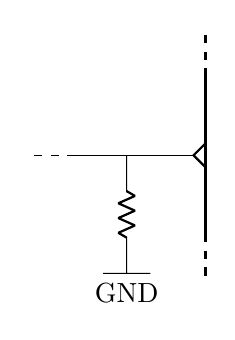
\begin{tikzpicture}
					\draw [very thick] (0,1) -- ++(0,-2);
					\draw [very thick, dashed] (0,1) -- ++(0,.6) (0,-1) -- ++(0,-.6);
					\draw [thick] (0,.15) -- ++(-.15,-.15) -- ++(.15,-.15);
					\draw (-.15,0) -- ++(-1.5,0)coordinate (i);
					\draw (-1,0) to[R,/tikz/circuitikz/bipoles/length=20pt] ++(0,-1.5) node[below]{GND} -- ++(-.3,0) --++(.6,0);
					\draw [dashed] (i) -- ++(-.6,0);
				\end{tikzpicture}
			\end{column}
		\end{columns}
	\end{frame}

	\begin{frame}
		\frametitle{Development phase - GPIOs}
		Internal circuit classification:
		\vspace{.3cm}
		\begin{columns}[T]
			\begin{column}{.5\textwidth}
				\centering
				\textbf{Push-pull}\\\vspace{.5cm}
				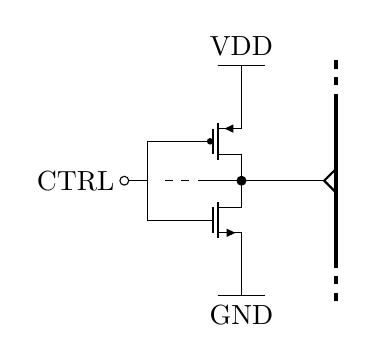
\begin{tikzpicture}
					\draw [very thick] (0,1) -- ++(0,-2);
					\draw [very thick, dashed] (0,1) -- ++(0,.6) (0,-1) -- ++(0,-.6);
					\draw [thick] (0,.15) -- ++(-.15,-.15) -- ++(.15,-.15);
					\draw (-.15,0)coordinate (in) -- ++(-1.5,0)coordinate (i);
					\node[nmos,scale=.6] (N) at (-1.2,-.5){};
					\node[pmos,scale=.6] (P) at (-1.2,.5){};
					\draw (N.drain) --(N.drain|-in) to [short,-*] ++(0,0) (N.source) -- ++(0,-.5) node[below]{GND} -- ++(-.3,0) -- ++(.6,0) (P.source) -- ++(0,.5) node[above]{VDD} -- ++(-.3,0) -- ++(.6,0) (N.gate) -- ++ (-.6,0)coordinate(A1) -- (P.gate-|A1) coordinate(A2) --(P.gate) ($(A1)!.5!(A2)$) to [short,-o] ++(-.3,0) node[anchor=east,left]{CTRL};
					\draw [dashed] (i) -- ++(-.6,0);
				\end{tikzpicture}
			\end{column}
			\begin{column}{.5\textwidth}
				\centering
				\textbf{Open drain}\\\vspace{.5cm}
				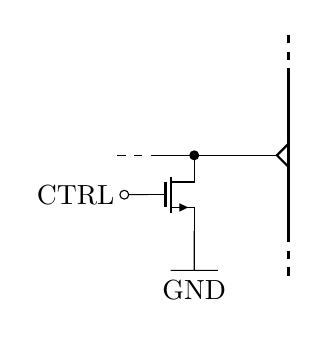
\begin{tikzpicture}
					\draw [very thick] (0,1) -- ++(0,-2);
					\draw [very thick, dashed] (0,1) -- ++(0,.6) (0,-1) -- ++(0,-.6);
					\draw [thick] (0,.15) -- ++(-.15,-.15) -- ++(.15,-.15);
					\draw (-.15,0)coordinate (in) -- ++(-1.5,0)coordinate (i);
					\node[nmos,scale=.6] (N) at (-1.2,-.5){};
					\draw (N.drain) --(N.drain|-in) to [short,-*] ++(0,0) (N.source) -- ++(0,-.5) node[below]{GND} -- ++(-.3,0) -- ++(.6,0) (N.gate) to [short,-o] ++(-.3,0) node[anchor=east,left]{CTRL};
					\draw [dashed] (i) -- ++(-.6,0);
				\end{tikzpicture}
			\end{column}
		\end{columns}	
	\end{frame}

	\begin{frame}
		\frametitle{Development phase - Peripheral configuration}
		\begin{columns}
			\begin{column}{.5\textwidth} 
				SPI configuration
				\centering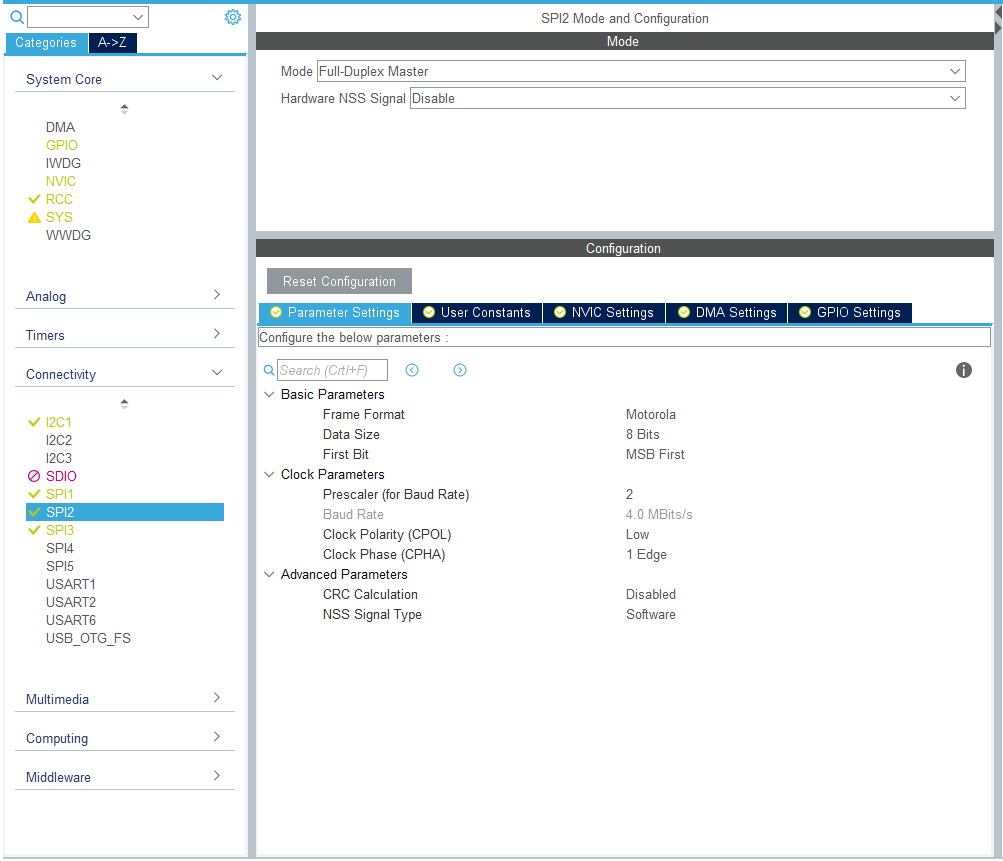
\includegraphics[width=\textwidth]{media/peripheral.png}
			\end{column}
			\begin{column}{.5\textwidth}
				I2C configuration
				\centering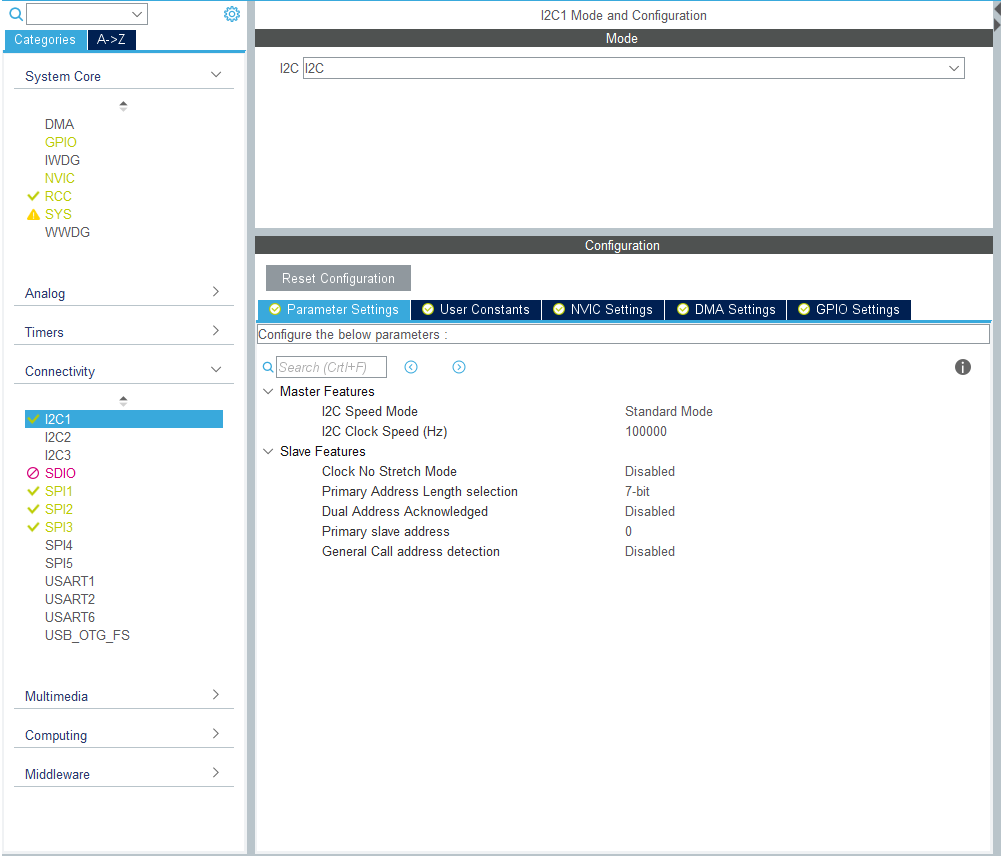
\includegraphics[width=\textwidth]{media/peripheral_2.png}
			\end{column}
		\end{columns}
		
	\end{frame}

	\begin{frame}
		\frametitle{Development phase - Clock tree}
		\centering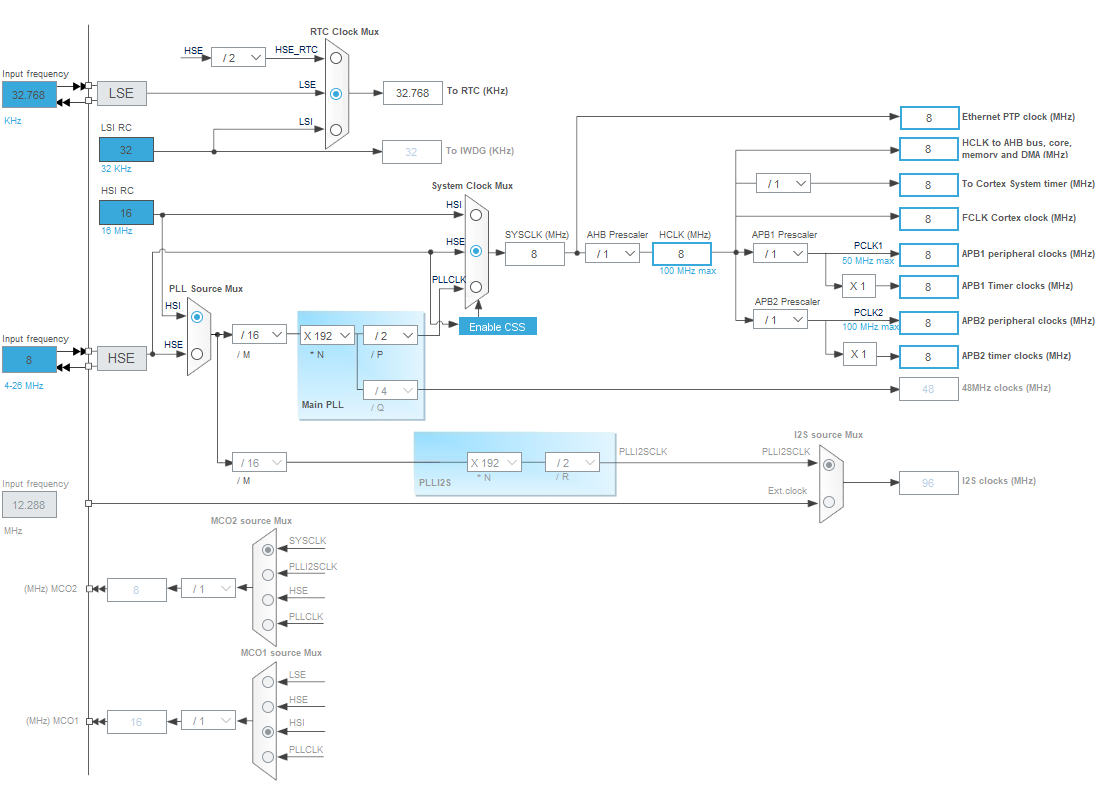
\includegraphics[width=.68\textwidth]{media/clock_tree.png}
	\end{frame}

	\begin{frame}
		\frametitle{Development phase - Clock tree glossary}
		\begin{description}
			\item[LSE] \textbf{L}ow \textbf{S}peed \textbf{E}xternal: microcontroller input for a low speed (\SI{32}{\kilo\hertz}) external oscillator.
			\item[HSE] \textbf{H}igh \textbf{S}peed \textbf{E}xternal: microcontroller input for a high speed (\SIrange{4}{26}{\mega\hertz}) external oscillator.
			\item[LSI] \textbf{L}ow \textbf{S}peed \textbf{I}nternal: internal RC oscillator for a \SI{32}{\kilo\hertz} clock.
			\item[HSI] \textbf{H}igh \textbf{S}peed \textbf{I}nternal: internal RC oscillator for a \SI{16}{\mega\hertz} clock.
			\item[PLL] \textbf{P}hase \textbf{L}ocked \textbf{L}oop: versatile circuit, used in this case as a frequency multiplier.
		\end{description}
	\end{frame}

	\begin{frame}
		\frametitle{Development phase - Finite State Machine}
		By definition from automata theory, a Finite State Machine is an abstract device that consists of:
		\begin{itemize}
			\item a [finite] set of \textbf{states}
			\item an alphabet ([finite] set) of \textbf{symbols} as possible inputs
			\item a \textbf{transition function} that takes an input symbol as parameter
		\end{itemize}
		A FSM is particularly useful to model simple systems that have a limited number of jobs (e.g. a traffic light). A simple representation of a FSM can be a state diagram or a state-transition table.
	\end{frame}

	\begin{frame}
		\frametitle{Development phase - State Diagram}
		A state diagram is a diagram usually describing the behavior of a system. It is represented or depicted as a directed graph.\\\vspace{.3cm}
		\centering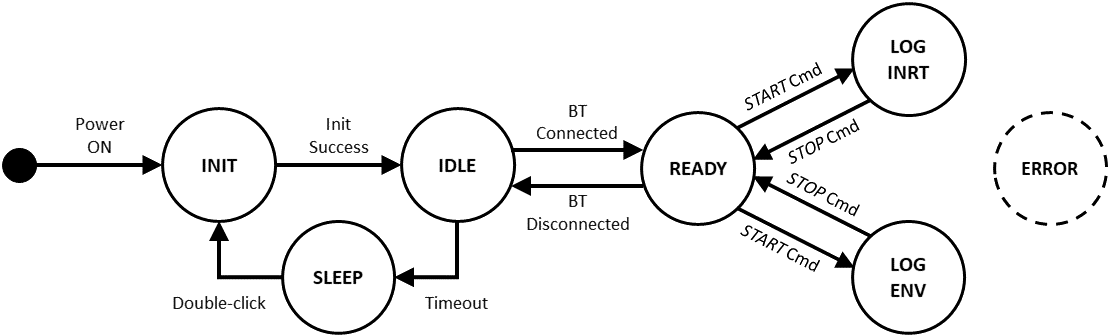
\includegraphics[width=.8\textwidth]{media/state_diagram.png}
	\end{frame}

	\begin{frame}
		\frametitle{Development phase - Event driven system behavior}
		A possible approach to firmware development is that of programming the system to be reactive to external events. To this end, it is best to define system states so that:
		\begin{itemize}
			\item two different states do not have the same job; a new state is better than two states sharing something in common;
			\item there is a clear event that defines the change from one state to the next.
		\end{itemize}
		
	\end{frame}

	\begin{frame}[fragile]
		\frametitle{Development phase - Event driven system behavior}
		Once the states have been defined, a function is executed periodically with a low priority. For example:\\
		\hspace{-3cm}\begin{adjustbox}{max width=.9\textwidth}
			\begin{lstlisting}[language=C]
				void doIdleJob(void){
					...
					//do stuff
					...
					//Maybe blink the LED to show that the system is alive
					...
				}
			
				void doReadyJob(void){
					...
					//do other stuff
					...
					//Blink the led some other color to show that the system is ready
					...
				}
			\end{lstlisting}
		\end{adjustbox}\\
		Events must then be defined as high priority functions (interrupt) that perform operations needed in the state change and start the new (low-priority) job.	
	\end{frame}

	\begin{frame}
		\frametitle{Development phase - Event driven system behavior}
		Other jobs, common to various states (USB, BT comm, ...) can \textbf{interrupt} the low priority \texttt{doXJob} function to execute. This leads to a system in which a single state logic is contained inside a single function, and external (or internal) events change the function executing at a given time.\\ In order for this system to work, priorities must be designed carefully.\\
		\vspace{.1cm}\centering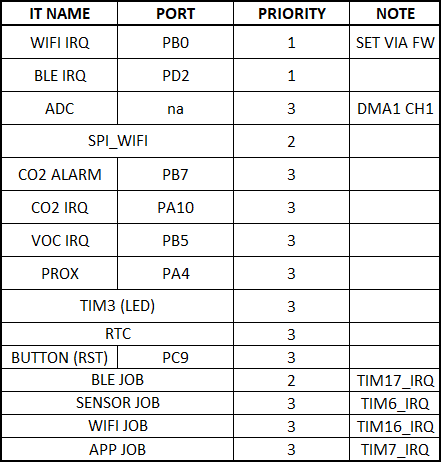
\includegraphics[width=.27\textwidth]{media/priorities.png}
	\end{frame}

	\begin{frame}
		\frametitle{Conclusions}
		\only<1>{
			\alert{Project phase}
			\begin{itemize}
				\item Specifications document is meant to concretize abstract requirements into concrete goals/limitations.
				\item Always try to minimize size, power consumption and cost if this does not hinder other requirements.
				\item Choose sensors, memory and comms according to specs, then choose microcontroller to fit.
				\item Choose battery and power management ICs after defining other system components to fit.
				
			\end{itemize}
		}
	
		\only<2>{
			\alert{Development phase}
			\begin{itemize}
				\item Rules rule the PCB: define ERD and DRC rules first.
				\item Define stackup of the PCB prior to design; assign planes.
				\item Prepare all components and footprints; triple check footprints designs.
				\item Take particular care in the placement of components; consider ease of routing and heat spots.
				
			\end{itemize}
		}
	
		\only<3>{
			\alert{Development phase}
			\begin{itemize}
				\item If possible, create the project to link hardware and firmware prior to PCB manufacture.
				\item Leave all unused pins as analog inputs (high impedance) to minimize microcontroller power consumption.
				\item Use the minimum clock that meets your requirements; avoid PLL if possible.
				\item Design FSM so that states functions do not overlap; make states transitions as concise as possible.
				\item Define job priorities early in the development. Changing them afterwards can be cumbersome.
			\end{itemize}
		}
	\end{frame}
	

\end{document}
